\chapter{Equazioni Differenziali}
\section{Preliminari}
Equazione è un uguaglianza in cui c'è almeno una incognita.\\
Equazione differenziale è un particolare tipo di equazione e stabilisce una relazione tra la funzione incognita e le sue derivate.In un equazione funzionale si cerca l'uguaglianza di: insieme di arrivo, insieme di partenza, corrispondenza.\\
Non è necessario sapere il valore della soluzione ma sapere che ne esiste una.????????\\\\
Equazione differenziale ordinaria:\\
1- La funzione incognita è funzione di una sola variabile, solitamente il tempo.\\
2- La funzione incognita e le sue derivate sono calcolate allo stesso istante di tempo.\\
\begin{definition}[Equazione differenziale]
	\label{def:equaz_diff}
	Si dice equazione differenziale ordinaria di ordine $n$ nella funzione incognita $x\in \R^k$ un espressione del tipo:
	$$f(t,x, x',\ldots,x^{(n)})=0$$
	dove $f:A\to \R^m$, $A\subseteq \R^{1+(1+n)k}$ e $t\in \R$.\\
	$m$ e $k$ caratterizzano il problema e son dunque libere. La dimensione di partenza $1+(1+n)k$ del problema è obbligata e dovuta alla somma di:
	\begin{itemize}
		\item $1 = dim(t)$
		\item $(1+n)k$
		\begin{itemize}
			\item $(1+n)$ il numero totale delle funzioni: $n$ derivate ed $x$ stessa
			\item $k$ la dimensione dell'insieme di partenza di ogni funzione incognita
		\end{itemize}
	\end{itemize}
	\textbf{Soluzione} di questa equazione differenziale è una qualunque funzione $x:I\to \R^k$ definita su un intervallo $I\subseteq \R$, derivabile $n$ volte in $I$ (e dunque continua in $I$) e tale che $\forall t\in I$
	$$t,x, x',\ldots,x^{(n)}) \in A$$
	$$f(t,x, x',\ldots,x^{(n)})=0$$
	\textbf{Soluzione massimale} di un equazione differenziale ordinaria è una soluzione $x_m:I_m\to \R^k$ tale che nessuna soluzione possa essere definita in un intervallo $I$ con $I_m\subseteq I$
\end{definition}
\begin{note} \hypertarget{def:equaz_diff_sol}{}
	Dalla definizione segue che $x \in \circdot{A}$, in quanto se non fosse in $\circdot{A}$ sarebbe di frontiera, ma un punto di frontiera non può essere derivabile.
\end{note}
\begin{note}
	Un'equazione differenziale ammette, in generale, infinite soluzioni.
\end{note}
\begin{note} \hypertarget{note:diff_eq_sol_definit_set}{}
	La soluzione di un'equazione differenziale può, analiticamente, essere definita su un intervallo $J\supset I$ ($I$ intervallo di definizione della funz. differenziale $f$). Non ha però senso considerare il suo comportamento al di fuori di $I$, in quanto non ha valore dal punto di vista del sistema. Per questo motivo $J$ sarà sempre considerato $J\subseteq I$
\end{note}
\begin{note}
	dalla \fullref{def:equaz_diff} segue che l'insieme di definizione della soluzione di un'equazione differenziale può essere solo un intervallo
\end{note}
\begin{example}
	Presa l'equazione differenziale $ x'=1$, essa è risolta da $x(t) = t + \alpha$ per ogni $\alpha\in\R$
\end{example}
\begin{exercise}
	La soluzione di un'equazione differenziale ordinaria non può avere 3 asintoti.
	\begin{solution}
		La soluzione $x$ è funzione continua. In quanto continua non può avere più di 2 asintoti verticali e in quanto funzione non può avere più di 2 asintoti orizzontali.
	\end{solution}
\end{exercise}
\definition
un'equazione differenziale è in forma normale  se e solo se si presenta nella forma 
$$x^{(n)} = g(t,x, x',\ldots,x^{(n-1)})$$
\observation
lo studio di un'equazione differenziale ordinaria in forma non normale inizia generalmente con l'utilizzo del Teorema della Funzione Implicita insieme ai teoremi sulle equazioni differenziali ordinarie in forma normale
\proposition\label{prop:equaz_n_equival_1}
ogni equazione differenziale ordinaria in forma normale di ordine $n$ è equivalente a una equazione differenziale ordinaria in forma normale di ordine $1$, cioè in cui compaiono solamente derivate prime.
\begin{proof}
	Data l'equazione
	$$x^{(n)} = g(t,x, x', x'',\ldots,x^{(n-1)})$$
	sia $y$ il vettore $y = \rvect{x &  x' &  x'' & \ldots & x^{(n-1)}}$. Abbiamo ora che le componenti del vettore sono
	$$y_1=x\qquad y_2= x'\qquad y_3= x''\qquad \ldots\qquad y_n=x^{(n-1)}$$
	ed al contempo
	$$y_1'= x'=y_2\qquad y_2'= x''=y_3\qquad y_3'= x'''=y_4\qquad\ldots\qquad y_{n-1}'=x^{(n-1)}=y_n$$
	Cioè, differenziando l'$i-esimo$ elemento (funzione) del vettore $y$, mi "sposto" all'elemento (funzione) $i+1$ di $y$. A questo punto tutti gli elementi di $y$ sono equazioni differenziali del primo ordine.\\
	Quindi l'equazione può essere scritta come il seguente sistema del primo ordine
	$$\begin{cases}y_1'\quad=\quad y_2\\y_2'\quad=\quad y_3\\\vdots\\y_n'\quad=\quad g(t, y_1, y_2,\dots,y_n)\end{cases}$$
\end{proof}
\begin{example}
	CASO n=2\\
	abbiamo che $ x''=f(t,x, x')$\\
	introduco $ X'=\begin{bmatrix} x'\\ x''\end{bmatrix}$ e $X=\begin{bmatrix}x\\ x'\end{bmatrix}$\\
	quindi $ X'=f(t,X)$
\end{example}
\begin{definition}[Problema di Cauchy del Primo Ordine]
	\label{def:prob_cauchy_ord_1}
	si dice problema di Cauchy del primo ordine il problema di determinare una soluzione di un'equazione differenziale ordinaria del primo ordine, soddisfacente ad una condizione iniziale.
	$$\begin{cases}x'=f(t,x)\\x(t_0)=x_0\end{cases}$$
	Dove $f:J\times A\to \R^n$, $J\subseteq \R$ è un intervallo, $t_0\in\circdot{J}$, $A\subseteq \R^n$, $x_0\in\circdot{A}$.\\
	Soluzione di un problema di Cauchy è una funzione $x:I\to \R^n$, definita in un intervallo $I$ contenente $t_0$ nella sua parte interna, quindi $t_0\in I\subseteq J$.\\
	Tale funzione $x$ è soluzione dell'equazione differenziale $x'=f(t,x)$ ed è tale che:
	\begin{enumerate}
		\item $x(t_0)=x_0$
		\item $x(I)\subseteq A$
		\item $x$ derivabile
	\end{enumerate}
	Quindi il problema di Cauchy aggiunge un vincolo ad un'equazione differenziale, così si isola una singola soluzione
\end{definition}
\begin{note}
	Si considera un intervallo perché l'idea è di studiare l'andamento nel tempo e sarebbe difficile far previsioni con "buchi" di tempo
\end{note}
\begin{note}
	La condizione $x(t_0) = x_0$ viene spesso definita condizione iniziale, malgrado la \fullref{def:prob_cauchy_ord_1} indichi che $t_0 \in \circdot{I}$, dunque a rigore non dovrebbe essere sulla frontiera di $I$. Questo è dovuto al fatto che, spesso, $t_0$ è proprio all'inizio dell'intervallo in cui si cerca la soluzione dell'equazione, ma i risultati esposti continuano a valere con piccole modifiche alle dimostrazioni.
\end{note}
\begin{definition}
	soluzione massimale di un problema di Cauchy è una soluzione $$x_M:I_M\mapsto R^k$$ tale che nessun'altra soluzione della stessa equazione possa essere definita in un intervallo $I$ con $I_M \subset I$. Quindi è la soluzione definita sull'intervallo maggiore possibile.
\end{definition}
\begin{definition}[Problema di Cauchy di Ordine $n$]
	si dice problema di Cauchy di ordine $n$ il seguente problema:\\
	Determinare una soluzione di un'equazione differenziale ordinaria di ordine $n$ soddisfacente a $n$ condizioni iniziali:
	$$\begin{cases}
		x^{(n)}=f(t,x,x',\dotsc,x^{(n-1)})\\
		x(t_0)=\alpha_0\\
		x'(t_0)=\alpha_1\\
		\vdots\\
		x^{(n-1)}(t_0)=\alpha_{n-1}
	\end{cases}$$
\end{definition}
\begin{note}
	Le condizioni iniziali devono essere assegnate tutte nello steso istante.
\end{note}
\begin{example}
	il problema di Cauchy $$\begin{cases}x'=x\\x(0)=1\end{cases}$$
	ammette, tra le altre, anche le seguenti soluzioni, tecnicamente distinte tra loro
	$$\funcdef{f_1}t[\realintervalclose{-1}{1}]{\R}[e^t] \qquad \funcdef{f_2}t[\realintervalclose{-2}{10}]{\R}[e^t]$$
	La soluzione massimale è
	$$\funcdef{f_M}t[\R]{\R}[e^t]$$
	con intervallo di partenza $\R$, avente evidentemente diametro maggiore possibile.
\end{example}
\begin{proposition}
	ogni problema di Cauchy di ordine $n$ è equivalente ad un problema di Cauchy del primo ordine
	\begin{proof}
		Dalla \fullref{prop:equaz_n_equival_1}
	\end{proof}
\end{proposition}
\begin{definition}[Equazione di Volterra]
	\label{def:equaz_volterra}
	Ogni problema di Cauchy del primo ordine con secondo membro continuo
	$$\begin{cases}x'=f(t,x)\\x(t_0)=x_0\end{cases}$$
	è equivalente ad un'equazione integrale del tipo
	$$x(t)=x_0+\int_{t_0}^{t}\Bigl(f\bigl(\tau,x(\tau)\bigr)\Bigr)\integrald{\tau}$$
	Questa equazione viene denominata \textbf{equazione integrale di Volterra}.
	\begin{proof}
		Integrando ambo i membri della prima equazione del problema di ottiene:
		$$\int_{t_0}^{t}( x')\integrald{\tau}=\int_{t_0}^{t}(f(\tau,x(\tau)))\integrald{\tau}$$
		$$x(t)-x(t_0)=\int_{t_0}^{t}(f(\tau,x(\tau)))\integrald{\tau}$$
		$$x(t)=x_0+\int_{t_0}^{t}(f(\tau,x(\tau)))\integrald{\tau}$$
	\end{proof}
	\begin{note}
		\hypertarget{note:volterra_non_cont}
		Questa equazione ha senso anche per alcune funzioni $f$ non non continue, ma solo misurabili nel primo argomento. Ne consegue che nei Teoremi di esistenza ed unicità (locali/globali) l'ipotesi ``$f$ continua'' può essere sostituita da ``$f$ continua a tratti in $t, \forall x$, continua in $x$ e limitata''.
	\end{note}
\end{definition}

\begin{observation}[Problema ben posto nel senso di Hadamard]
	\label{obs:hadamard}
	in generale un problema si dice \textbf{ben posto} o \textbf{ben posto nel senso di Hadamard} ogniqualvolta la soluzione:
	\begin{enumerate}
		\item esiste
		\item è unica
		\item dipende con continuità dai dati
	\end{enumerate}
\end{observation}

\section{Teoria Locale}
\begin{definition}[Funzione localmente Lipschitziana]
	\label{def:loc_lips}
	Una funzione $f:I\times A\to \R^n$, con $I$ intervallo in $\R$ e $A$ aperto in $\R^n$, si dice \textbf{localmente lipschitziana} in $x\in A$ \textbf{uniformemente} rispetto a $t$ se
	$$\forall x_0 \in A, \exists r>0 e L>0: \forall x_1,x_2 \in (B(x_0,r)\cap A), \forall t\in I$$
	vale che
	$$\norm{f(t,x_2)-f(t,x_1)}\leq L\cdot\norm{x_2-x_1}\qquad o, ugualmente\qquad\frac{\norm{f(t,x_2)-f(t,x_1)}}{\norm{x_2-x_1}}\leq L$$
	Una funzione è uniformemente lipschitziana (\textbf{unif. lips.}) in un'intervallo $I$ se, in parole povere, è possibile individuare per ogni punto di $I$ una sfera $B$ in cui la funzione è lipschitziana.
\end{definition}
\begin{note}
	La località è data da $x_1,x_2 \in (B(x_0,r)\cap A)$ e l'uniformità da $\forall t\in I$. Quindi la $f$ rimane lips. in modo uniforme al variare di $t$ (cioè $\forall t\in I$), ma questo non è garantito $\forall x\in A$, solo per $x_1,x_2 \in (B(x_0,r)\cap A)$.
\end{note}
\begin{note}
	\hypertarget{note:if_lips_then_loclips}
	Se $f$ \textbf{lips} su $A\implies f$ \textbf{loc. lips.} su A
\end{note}
\begin{proposition}
	\label{prop:fc1_loc_lips}
	Siano $I\subseteq \R$ un intervallo aperto e $A\subseteq \R^n$ un aperto. Ogni funzione $f\in\cntclass{1}(I\times A;\R^n)$ è loc. lips. in $x\in A$ uniformemente rispetto a $t\in I$
	\begin{proof}
		Il prodotto cartesiano $I\times A$, essendo prodotto cartesiano di aperti in $\R^n$ con metrica euclidea (si suppone sia in uso questa metrica), è a sua volta un aperto. Questo risultato è dovuto alla definizione stessa del prodotto cartesiano di $\R$ con metrica euclidea.\\
		% TODO scrivere proposizione poligonale capitolo 1. Magari anche proposizione prodotto cartesiano di aperti = aperto.
		Chiamiamo ora $S=I\times A$ l'insieme di partenza della $f$. Grazie alla \fullref{prop:polig_cong_aperto} sappiamo che esiste una poligonale interamente contenuta in $S$ congiungente due qualunque punti dell'aperto $S$.\\
		È ora possibile applicare il \fullref{teo:accresc_fin} ad uno qualunque dei segmenti formanti la poligonale appena individuata. Vale quindi la
		$$\norm{f(x_1)-f(x_0)}\le \sup\limits_{x\in S}\norm{Df(x)}\norm{x_1-x_0}$$
		che è direttamente comparabile alla \fullref{def:loc_lips} della funzione in ciascuno dei segmenti della poligonale, da cui la tesi.
	\end{proof}
\end{proposition}
\begin{example}
	La funzione $f:\R\mapsto\R$ data da $f(x)=x^2$ è \textbf{loc. lips.} su $\R$ ma non è \textbf{globalmente lips.} su $\R$. Vedasi \fullref{def:lips}
\end{example}

\subsection{Esistenza e Unicità}
\begin{proposition}[Teorema di Peano]
	\label{teo:peano}
	Si consideri il seguente problema di Cauchy:
	$$\left\{\begin{matrix} x'=f(t,x)\\x(t_0)=x_0\end{matrix}\right.$$
	con $f:I\times A\in \R^n$ soddisfacente alle ipotesi:
	\begin{enumerate}
		\item $t_0\in \circdot{I}, x_0\in \circdot{A}$
		\item $f\in \cntclass{0}(I\times A;R^n)$
	\end{enumerate}
	inoltre $I\subseteq \R$ intervallo e $A\subseteq \R^n$, per \fullref{def:prob_cauchy_ord_1}.\\
	Allora esiste un $\delta>0$ tale che esiste soluzione $x:J\mapsto A$ del problema di Cauchy con $J=\realintervalclose{t_0-\delta}{t_0+\delta}$.
	\begin{note}
		$\delta$ è un valore arbitrario che serve ad identificare l'intervallo $I$ a cui appartiene $t_0$
	\end{note}
	\noindent Inoltre:
	\begin{itemize}
		\item $J\subseteq I$ da \hyperlink{note:diff_eq_sol_definit_set}{nota definizione 47}, dunque $\varphi(J)\subseteq A$
		\item $\varphi(t_0)=x_0$
		\item $\varphi$ derivabile e $\varphi'(t)=f(t,\varphi(t))$
	\end{itemize}
	\begin{proof}
		Non richiesta
	\end{proof}
\end{proposition}
\begin{example}[Il Baffo/Pennello di Peano] % TODO da rivedere
	$$\left\{\begin{matrix} x'=\sqrt{\abs{x}}\\x(0)=x_0\end{matrix}\right.$$
	\begin{center}
		\begin{tikzpicture}[scale=1] %[x={10.0pt},y={10.0pt}]
		\pgfmathsetmacro\MAX{2}
		\draw[->] (-\MAX,0) -- (\MAX,0) node[anchor=north west] {x};
		\draw[->] (0,-\MAX) -- (0,\MAX) node[anchor=south east] {$ x'$};
		\draw[domain=0:2,smooth,variable=\x] plot ({\x},{(\x)^(1/2)});
		\draw[domain=-2:0,smooth,variable=\x] plot ({\x},{(-\x)^(1/2)});
		%\draw node at (0.5,0) {$|$};
		%\draw node at (1,0) {$|$};
		%\draw node at (1.5,0) {$|$};
		%\draw node at (0,0.5) {$-$};
		%\draw node at (0,1) {$-$};
		%\draw node at (0,1.5) {$-$};
		%\draw node[anchor=north] at (0.5,0) {$x_0$};
		%\draw node[anchor=north] at (1,0) {$x_0+h$};
		%\draw node[anchor=north] at (1.5,0) {$x_0+2h$};
		%\draw node[anchor=east] at (0,0.5) {$ x'' $};
		%\draw node[anchor=east] at (0,1) {$ x''' $};
		%\draw node[anchor=east] at (0,1.5) {$ x''''$};
		
		\end{tikzpicture}% pic 1
		\qquad % <----------------- SPACE BETWEEN PICTURES
		\begin{tikzpicture}[scale=1] %[x={10.0pt},y={10.0pt}]
		\pgfmathsetmacro\MAX{2}
		\draw[->] (-\MAX,0) -- (\MAX,0) node[anchor=north west] {t};
		\draw[->] (0,-\MAX) -- (0,\MAX) node[anchor=south east] {x};
		\end{tikzpicture}% pic 2
	\end{center}
	Se $x_0 = 0$ ho che $\varphi(t)=0$ è soluzione $\forall t$\\
	Ma $x' = \sqrt{\abs{x}}$ è anche un'equazione a variabili separabili, quindi risolvibile.
	$$\frac{x}{\sqrt{\abs{x}}}=1 \Rightarrow \int_{0}^{t}{\frac{ x'}{\sqrt{\abs{x}}}\integrald{t}} = t$$
	$$\int_{x(0)=0}^{x(t)}{\frac{1}{\sqrt{\abs{x}}}\integrald{x}} = t$$
	valuto ora il caso $x\geq0$, quindi $\abs{x}=x$
	$$\int_{x(0)=0}^{x(t)}{\frac{1}{\sqrt{x}}\integrald{x}} = 2\sqrt{x} = t$$
	La soluzione cercata è quindi $x(t)=\frac{1}{4}t^2$, estendendo il ragionamento ai tempi negativi si trova che la soluzione cercata è: $$\varphi(x)= \left\{\begin{matrix}+\frac{1}{4}t^2&&t>0,\\0&&t=0\\-\frac{1}{4}t^2&&t<0\end{matrix}\right.$$
	Abbiamo trovato che per la condizione iniziale $x_0=0$ il sistema ammette due soluzioni, si riesce estendere la soluzione a infinite funzioni.
	$$\varphi(x)= \left\{\begin{matrix}-\frac{1}{4}(t-a)^2&&t<a,\\0&&t\in[a,b]\\+\frac{1}{4}(t-b)^2&&t>b\end{matrix}\right.$$
	infatti:
	$$\varphi'(t) = \left\{\begin{matrix}-\frac{1}{8}(t-a)&&t<a,\\0&&t\in[a,b]\\+\frac{1}{8}(t-b)&&t>b\end{matrix}\right.$$ $$\left\{\begin{matrix}-\frac{1}{8}(t-a)=\frac{-\frac{1}{4}(t-a)^2}{	\sqrt{-\frac{1}{4}(t-a)^2}}&&t<a,\\0=0&&t\in[a,b]\\+\frac{1}{8}(t-b)=\frac{\frac{1}{4}(t-b)^2}{\sqrt{\frac{1}{4}(t-b)^2}}&&t>b\end{matrix}\right. = ....????? sistema $$
	Abbiamo quindi trovato infinite soluzioni.\\
	Questo esempio per sottolineare che il teorema di Peano non garantisce l'unicità della soluzione
\end{example}
\begin{example}[Continuità ed ipotesi necessaria] % TODO da rivedere
	Questo esempio mostra che se non c'è continuità, può?????????? non esserci la soluzione.\\
	Dato il seguente problema di Cauchy: $\left\{\begin{matrix}
	x' = \left\{\begin{matrix}1&&x<0\\-1&&x\ge 0\end{matrix}\right.\\
	x(0)=0
	\end{matrix}\right.$\\
	\begin{center}
		\begin{tikzpicture}[scale=1] %[x={10.0pt},y={10.0pt}]
		\pgfmathsetmacro\MAX{2}
		\draw[->] (-\MAX,0) -- (\MAX,0) node[anchor=north west] {x};
		\draw[->] (0,-\MAX) -- (0,\MAX) node[anchor=south east] {$ x'$};
		\draw[domain=0:2,smooth,variable=\x] plot ({\x},{1});
		\draw[domain=-2:0,smooth,variable=\x] plot ({\x},{-1});
		\draw node at (0,-1) {$\bullet$};
		\draw node at (0,1) {$\circ$};
		\end{tikzpicture}% pic 1
	\end{center}

	\noindent $x(t)=0$ soddisfa la condizione iniziale ma ovviamente non può essere soluzione del problema poiché per $x\ne 0$ si ha che $ x'=\pm 1$ che non è la derivata della funzione nulla.\\
	partendo sempre dalla condizione iniziale si può ipotizzare per esempio che la soluzione cresca, solo che questo contraddice $ x'(0)=-1$\\
	se invece si ipotizza che decresce da $0$ si ottiene che la funzione assume valori negativi, anche questo è un assurdo poiché la derivata per valori negativi della funzione è positiva.\\
	Precisiamo che se il problema fosse stato $\left\{\begin{matrix}
	x' = \left\{\begin{matrix}1&&x<0\\-1&&x\ge 0\end{matrix}\right.\\
	x(0)=-3\end{matrix}\right.$ allora la funzione $\varphi(x)=-x+3$ sarebbe stata soluzione nell'intervallo $J=\left] -\infty,0 \right[ $
\end{example}

\begin{theorem}[Teorema di Cauchy Locale - Prima Parte]
	\label{teo:cau_locale_part_1}
	Si consideri il problema di Cauchy:
	$$\begin{cases}x'=f(t,x)\\x(t_0)=x_0\end{cases}$$
	con $f:I\times A \to \R^n$ soddisfacente le ipotesi:
	\begin{enumerate}
		\item $t_0\in \circdot{I},\:x_0\in \circdot{A}$. Inoltre da \fullref{def:equaz_diff} e note successive: $I$ intervallo e $I\subseteq \R^n$, inoltre $A\subseteq \R^n$
		\item $f\in \cntclass{0}(I\times A; \R^n)$ 
		\item $f$ è localmente Lipschitziana in $x\in A$ uniformemente rispetto a $t\in I$
	\end{enumerate}
	\begin{note}
		Le prime due ipotesi garantiscono l'esistenza, grazie al \fullref{teo:peano}. La terza ipotesi rende il teorema più restrittivo, ma permette anche di giungere ad una conclusione più forte (ed utile).
	\end{note}
	\vspace*{-5ex}
	\begin{note}
		Per verificare l'ultima ipotesi si ricordino \fullref{prop:fc1_loc_lips} e \hyperlink{note:if_lips_then_loclips}{se $f$ \textbf{lips.} $\implies f$ \textbf{loc. lips.}}
	\end{note}
	Allora ho i seguenti risultati:
	\begin{enumerate}
		\item \textbf{Esistenza}:\\
		da \fullref{teo:peano} $\exists \delta>0$, con cui si identifica un $J=\realintervalclose{t_0-\delta}{t_0+\delta}$. Inoltre $\exists\,\varphi : J \to \R^n$ è soluzione con le proprietà date da Peano:
		\begin{itemize}
			\item $J\subseteq I$ da \hyperlink{note:diff_eq_sol_definit_set}{nota definizione 47}, dunque $\varphi(J)\subseteq A$
			\item $\varphi(t_0)=x_0$
			\item $\varphi$ derivabile e $\varphi'(t)=f(t,\varphi(t))$
		\end{itemize}
		\item \textbf{Unicità}\\
		Se $\exists\,J_1,J_2$ intervalli con $J_1\subseteq I,J_2\subseteq I$ e $\exists\,\varphi_1:J_1\to \R^n, \varphi_2:J_2\to \R^n$ soluzioni con le seguenti proprietà
		\begin{itemize}
			\item $J_1\subseteq I$, $J_2\subseteq I$ da \hyperlink{note:diff_eq_sol_definit_set}{nota definizione 47}, dunque $\varphi_1(J_1)\subseteq A$ e $\varphi_2(J_2)\subseteq A$
			\item $\varphi_1(t_0)=x_0,\,\varphi_2(t_0)=x_0$
			\item $\varphi_1,\varphi_2$ derivabili e
				$\begin{cases}
					\varphi_1'(t)=f(t,\varphi_1(t))\,\forall t \in J_1\\
					\varphi_2'(t)=f(t,\varphi_2(t))\,\forall t \in J_2
				\end{cases}$
				NB. Non è effettivamente sistema
		\end{itemize}
		\begin{note}
			Si può osservare che, sicuramente, $J_1\cap J_2\neq\emptyset$, poiché entrambi gli insiemi contengono almeno $t_0$ nella loro parte interna.
		\end{note}
		Allora $\varphi_1(t)=\varphi_2(t)$\quad$\forall t \in(J_1\cap J_2)$\\
		Cioè, se esistono due soluzioni, allora esse coincidono ovunque siano entrambe definite.
		\item \textbf{Dipendenza continua dai dati}\\
		Questa tesi verrà esposta successivamente in \fullref{teo:cau_locale_part_2}
	\end{enumerate}
	\begin{proof}(\textbf{Tesi 2})
		\begin{note}
			L'idea alla base della dimostrazione è che vogliamo riuscire a trasformare il problema di Cauchy in un problema di punto fisso mediante una funzione avente come parametro $x$ stesso.
		\end{note}
		Da \fullref{def:equaz_volterra} sappiamo che la prima equazione del problema in ipotesi corrisponde all'integrale
		$$x(t)=x_0+\int_{t_0}^{t}\Bigl(f\bigl(\tau,x(\tau)\bigr)\Bigr)\integrald{\tau}$$
		Definiamo quindi $T$, funzione del tipo
		\begin{equation}
			\label{eq:cauch_proof_T}
			\funcdef{\textrm{$T$}}{\bigl(T(x)\bigr)(t)}{X}[x_0+\int_{t_0}^tf\bigl(\tau,x(\tau)\bigr)\integrald{\tau}]
		\end{equation}
		Abbiamo così ottenuto un problema di punto fisso ($x=T(x)$). Ora bisogna determinare l'insieme di partenza e l'insieme di arrivo in maniera utile per la dimostrazione. Per poter applicare il \fullref{teo:contrazioni} serve che lo spazio di partenza e di arrivo corrispondano.\\
		Prendiamo:
		\begin{itemize}
			\item $\delta_1>0$ tale che $\realintervalclose{t_0-\delta_1}{t_0+\delta_1}\subseteq I$
			\item $\rho>0$ tale che $\overline{B(x_0,\rho)}\subseteq A$
			\item $L$ costante di Lipshitz di $f$ in $\realintervalclose{t_0-\delta_1}{t_0+\delta_1}\times\overline{B(x_0,\rho)}$. È possibile individuare $L$ in quanto $f$ loc. lips. per ipotesi in $I\times A$, e dunque \textbf{loc. lips. in sottointervalli/insiemi}
		\end{itemize}
		Sia ora
		$$V = \sup\brackets{\norm{f(t,x)}\,:\,t\in\realintervalclose{t_0-\delta_1}{t_0+\delta_1},x\in\overline{B(x_0,\rho)}}$$
		\begin{note}
			V è il maggiore tra i valori assunti dalla derivata prima $\bigl(x'=f(t,x)\bigr)$ di una qualsiasi delle soluzioni $x$ contenute nella sfera $\overline{B(x_0,\rho)}$. È massimo di funzione continua (per ipotesi 2) in un compatto (per ipotesi 1, essendo in $\R^n\times\R^n$ e per \fullref{prop:int_compatto}).\\% TODO in cap. 1, prop 2.35: compatto <=> chiuso+limtato (intervallo)
		\end{note}
		\noindent Definiamo dunque un generico $\delta>0$
		\begin{equation}
			\label{eq:cau_delta}
			\delta<\min\brackets{\delta_1,\frac{\rho}{V},\frac{1}{L}}
		\end{equation}
		\begin{note}
			$\delta$ è strettamente minore del $\min$ perché poi servirà a trovare una contrazione, dunque dovrò avere sicuramente $\delta L < 1$
		\end{note}
		\begin{itemize}
			\item $\delta_1$ è raggio di un generico intervallo incluso in $I$ di partenza. $\delta$ deve essere minore di $\delta_1$ in quanto non è possibile uscire dall'intervallo $I$
			\item $\frac{\rho}{V}$ è rapporto tra il raggio di $\overline{B(x_0,\rho)}$, sfera interamente contenuta in $A$, e $V$, valore massimo di $f$ ridotta all'intervallo di cui sopra e alla sfera $\overline{B}$.\\
			Considerando il reciproco $\frac{V}{\rho}$, possiamo vederlo come una sorta di nuova costante di lips., riportata ad un intervallo più piccolo, non dipendente però da $\Delta f(x)$, ma dal valore di $f(x)$ stessa.
			\item $1/L = \frac{\norm{x_2-x_1}}{\norm{f(t,x_2)-f(t,x_1)}}$ dalla \fullref{def:loc_lips}, perché $f$ loc. lips. per ipotesi. Dà un'idea di quanto vari la $x$ rispetto alla variazione della $f(x)$
		\end{itemize}
		Questo $\delta$, dunque, rappresenta, dal punto di vista concettuale, quale sia la più restrittiva ($\min$) tra tutte le possibili variazioni della $f(x)$ rispetto alla $x$.\\
		A questo punto, usando $\delta$, definiamo lo spazio $X$, generato da tutte le funzioni continue sul nuovo intervallo a valori entro una sfera centrata in $x_0$ con lo stesso raggio di $\overline{B}$
		$$X = \brackets{g\in \cntclass{0}(\realintervalclose{t_0-\delta}{t_0+\delta};\R^n):\forall t\norm{g(t)-x_0}\leq \rho}$$
		\begin{note}
			Si scelgono le funzioni continue ($\in \cntclass{0}$) perché serve $x$ continua per rendere valida l'equivalenza della funzione di Volterra con il problema di Cauchy. Stando alla \hyperlink{note:volterra_non_cont}{nota alla definizione di equazione di Volterra} sarebbe possibile sceglierla non continua, ma non si considera il caso.
		\end{note}
		Possiamo passare al punto chiave della dimostrazione, verifichiamo le ipotesi del \fullref{teo:contrazioni}:
		\begin{itemize}
			\item $(X,d)$ è \textbf{spazio metrico completo}\\
			$(X,d_X)$ è spazio metrico completo se considerato con la distanza della convergenza uniforme $d_X = d_{\cntclass{0}}$ per il \fullref{prop:compl_dist_spm_compl}.\qed
			\item $T$ è \textbf{definita} (è possibile calcolarla)\\
			L'abbiamo definita all'inizio dall'equazione di Volterra\qed
			\item $T$ è \boldmath$X\mapsto X$\unboldmath\\
			L'insieme di partenza è valido in quanto sottoinsieme dell'insieme su cui $f(t,xt)$ era definita.\\
			Per verificare che $y=T(x)$, bisogna verificare che $y\in \cntclass{0}(\realintervalclose{t_0-\delta}{t_0+\delta};\R^n)$ e che $y(t)\in \overline{B(x_0,\rho)}\;\;\forall t \in \realintervalclose{t_0-\delta}{t_0+\delta}$
			\begin{proof}
				$y\in \cntclass{0}$ nell'intervallo specificato per il Teorema Fodamentale del Calcolo Integrale.\\
				La seconda condizione si verifica prendendo la \cref{eq:cauch_proof_T} e calcolando la norma di entrambi i termini
				\begin{align*}
					\norm{y(t)-x_0} &= \norm{\int_{t_0}^t f(\tau,x(\tau))\integrald{\tau} }
					\intertext{posso ora minorare con il valore assoluto della norma dell'argomento (spiegazione in \fullref{ex:cau_loc_abs_of_norm})}
					&\leq \abs{\int_{t_0}^t \norm{f(\tau,x(\tau))}\integrald{\tau} } \tageq\label{eq:cau_loc_abs_of_norm}
					\intertext{$\norm{f(\tau,x(\tau))}$ è sicuramente minorato da $V$ per definizione di quest'ultimo, dunque si ha integrale di costante}
					&\leq V \cdot \abs{t-t_0}
					\intertext{$\abs{t-t_0}\leq \delta$ per definizione di $\delta$}
					&\leq V \cdot \delta\\
					\intertext{nel caso in cui $\min\brackets{\delta_1,\frac{\rho}{V},\frac{1}{L}} = \frac{\rho}{V}$, allora minorato strettamente da $\rho$ per definizione di $\delta$, altrimenti sicuramente minore per $\min$}
					&< \rho
				\end{align*}
			\end{proof}
			\item $T$ è \textbf{contrazione}\\
			Occorre verificare la \cref{eq:def_contrazione}
			\begin{proof}
			Per definizione della $T$ e per la proprietà addittiva degli integrali
			\begin{align*}
				\bigl(T(x_2)\bigr)(t) - \bigl(T(x_1)\bigr)(t) =
				\int_{t_0}^t \Bigl(
					f\bigl(\tau,x_2(\tau)\bigr) - f\bigl(\tau,x_1(\tau)\bigr)
				\Bigr)\integrald{\tau}
			\end{align*}
			Dunque, passando alla norma di quanto calcolato sopra
			\begin{align}
				\norm{\bigl(T(x_2)\bigr)(t) - \bigl(T(x_1)\bigr)(t)} \label{eq:cau_loc_verif_contraz_norm}
			\end{align}
			È sicuramente minorata da
			\begin{align*}
				&\leq \abs{\int_{t_0}^t
					\norm{f\bigl(\tau,x_2(\tau)\bigr) - f\bigl(\tau,x_1(\tau)\bigr)}
					\integrald{\tau}}\\
				\intertext{Per \fullref{def:loc_lips} passo alle funzioni incognite $x_i$ di $f$ (che son le soluzioni dell'equazione differenziale), minorando}
				&\leq \abs{\int_{t_0}^t
					L\cdot\norm{x_2(\tau)-x_1(\tau)}
					\integrald{\tau}}\\
				\intertext{Dalla \fullref{obs:dist_conv_unif}, $\norm{f-g}_{\cntclass{0}} = \sup_A \abs{f-g} = d_{\cntclass{0}}(f,g)$}
				&= \abs{\int_{t_0}^t % WARNING qui nella dimostrazione sul libro c'è un <=, anche se non so perché
					L\cdot d_X(x_2,x_1)
					\integrald{\tau}}\\
				&= L \cdot \abs{t-t_0} \cdot d_X(x_2,x_1) \tageq\label{eq:cau_loc_verif_contraz_fine} % WARNING qui nella dimostrazione sul libro c'è un <=, anche se non so perché
			\end{align*}
			Quindi, concludendo, possiamo passare dalla \cref{eq:cau_loc_verif_contraz_norm} alla distanza $d_X$, semplicemente per definizione della distanza, cioè
			$$\norm{\bigl(T(x_2)\bigr)(t) - \bigl(T(x_2)\bigr)(t)} = d_X\bigl(T(x_2),T(x_1)\bigr)$$
			Minoriamo questa distanza con la forma appena trovata \cref{eq:cau_loc_verif_contraz_fine}. Per quanto riguarda $\abs{t-t_0}$, passiamo al $\sup$ di $t$ nell'intervallo $\realintervalclose{t_0-\delta}{t_0+\delta}$, cioè $\delta$ stesso
			$$d_X\bigl(T(x_2),T(x_1)\bigr) \leq (\delta \cdot L) \cdot d_X(x_2,x_1)$$
			Essendo, per definizione, $\delta$ al più pari ad $\frac{1}{L} \implies \delta\cdot L<1 \implies T$ è contrazione per \fullref{def:contrazione}.
			\end{proof}
		\end{itemize}
		È ora possibile applicare il \fullref{teo:contrazioni} che garantisce l'\textbf{unicità} del punto fisso $x_* \in X$ per la $x = T(x)$, questo implica ovviamente che $T(x)$ abbia un'unica soluzione. Si ha dunque l'unicità della soluzione $x$ del problema di Cauchy in ipotesi sull'intervallo $\realintervalclose{t_0-\delta}{t_0+\delta}$, al quale $T$ è equivalente per definizione in quanto $T$ è \fullref{def:equaz_volterra}.

		Tornando ai $J_1, J_2$ della Tesi 2:
		\begin{itemize}
			\item Se $(J_1 \cap J_2) \subseteq \realintervalclose{t_0-\delta}{t_0+\delta}$, allora $x_1 = x_2$ in quanto esiste unico punto fisso, come dimostrato sopra.
			\item Se $(J_1 \cap J_2) \supset \realintervalclose{t_0-\delta}{t_0+\delta}$, allora poniamo
				\begin{equation}
					t_M = \sup \brackets{t \in (J_1 \cap J_2): \forall \tau \in \realintervalclose{t_0}{t}, x_1(\tau)=x_2(\tau)}\label{eq:cau_loc_tM_J1J2_supset}
				\end{equation}
				$$x_M = x_1(t_M) = x_2(t_M)$$
				Quindi $t_M$ è l'\textit{ultimo istante} in cui $x_1$ e $x_2$ coincidono.

				Essendo
				\begin{itemize}
					\item $t_M \in \circdot{J_1},\,t_M \in \circdot{J_2} \implies t_M \in \circdot{I}$ da \hyperlink{note:diff_eq_sol_definit_set}{nota definizione 47}
					\item $x_M \in \circdot{A}$ per \hyperlink{def:equaz_diff_sol}{nota definizione equazione differenziale}
				\end{itemize}
				ci ritroviamo nelle ipotesi di quanto appena dimostrato, solo che con dei nuovi $t$ ed $x$. Possiamo dunque giungere alla conclusione che il problema di Cauchy
				$$\begin{cases}x'=f(t,x)\\x(t_M)=x_M\end{cases}$$
				ammetta unica soluzione definita in un intorno di $t_M$ del tipo $\realintervalclose{t_M-\delta}{\boldsymbol{t_M+\delta}}$, cioé $x_1$ e $x_2$ coincidono in un intorno di $t_M$. Il fatto che esista un'unica soluzione oltre $t_M$ (vedere parte in grassetto dell'intorno sopra) contraddice la \cref{eq:cau_loc_tM_J1J2_supset}, perché non dovrebbe essere possibile trovare una soluzione in comune \textit{oltre} $t_M$ per come è definito. Ripetendo iterativamente questo procedimento si può semplificare la definizione di $t_M$ a
				$$t_M = \min \brackets{\sup J_1, \sup J_2}$$
				Ripetendo quanto fatto con il \textit{primo istante} $t_m$ in cui $x_1$ e $x_2$ coincidono, si ottiene
				$$t_m = \max \brackets{\inf J_1, \inf J_2}$$
				Quindi, prendendo $\realintervalclose{t_m}{t_M}$, abbiamo identificato $J_1 \cap J_2$ stessa.
		\end{itemize}
		Dunque $x_1$ e $x_2$ coincidono in $J_1 \cap J_2$, indipendente dalla relazione tra intersezione e intervallo.
	\end{proof}
	\begin{note}
		La scelta di $\delta$ in \cref{eq:cau_delta} potrebbe essere migliorata utilizzando il \fullref{teo:iterata_contraz} e scegliendo $\delta<\min\brackets{\delta_1,\frac{\rho}{V}}$, indipendentemente dalla costante di lips. della $f$
		% TODO magari la dimostrazione?
	\end{note}
\end{theorem}

\begin{exercise}
	\label{ex:cau_loc_abs_of_norm}
	È necessario il modulo in \cref{eq:cau_loc_abs_of_norm}?
	\begin{solution}
		Consideriamo, ad esempio
		\begin{align*}
			&f(x) = \norm{\int_0^6 10\cdot\frac{\sin{x}}{1+x} \integrald{x}} = 4,9413 && \text{(sinistra)}\\
			&g(x) = \abs{\int_0^6 \norm{10\cdot\frac{\sin{x}}{1+x}} \integrald{x}} = 11,935 && \text{(destra)}
		\end{align*}
		Nella $f$, viene calcolata la norma del risultato dell'integrazione definita.\\
		Nella $g$ si ha invece la norma della funzione, cioè la parte "sotto l'asse $x$" della funzione viene ribaltata sopra l'asse dall'operatore norma, come si può vedere dal grafico. Questo implica che il valore della $g$ sarà sicuramente $\geq$ rispetto alla $f$, in quanto l'integrale è somma di soli infinitesimi positivi.\\
		Infine, il valore assoluto nella \cref{eq:cau_loc_abs_of_norm} è necessario per evitare che, scambiando gli estremi d'integrazione, si ottenga un valore negativo, che non potrebbe mai essere risultato del primo integrale
		\begin{center}
			\begin{tikzpicture}[baseline]
			\begin{axis} [
				width=\textwidth / 2 - 10,
				height=\textwidth / 2 - 10,
				axis lines = center,
				axis on top=true,
				axis equal,
				ymin = -2,
				xlabel = $x$,
				ylabel = {$f(x)$},
			]
				\addplot [
					name path=f,
					domain=0:7,
					samples=100,
					color=red,
				]
				{10*sin(deg(x))/(1+x)};
				\addlegendentry{\raisebox{.5ex}{$10\cdot\frac{\sin{x}}{1+x}$}}
		
				\path[name path=axis] (axis cs:\pgfkeysvalueof{/pgfplots/xmin},0) -- (axis cs:\pgfkeysvalueof{/pgfplots/xmax},0);
				\addplot[red!30] fill between[of=f and axis, soft clip={domain=0:6}];
			\end{axis}
			\end{tikzpicture}
			~\qquad\qquad
			\begin{tikzpicture}[baseline]
			\begin{axis} [
				width=\textwidth / 2 - 10,
				height=\textwidth / 2 - 10,
				axis lines = center,
				axis on top=true,
				axis equal,
				ymin = -2,
				xlabel = $x$,
				ylabel = {$g(x)$},
			]
				\addplot [
					name path=g,
					domain=0:7,
					samples=100,
					color=blue,
				]
				{abs(10*sin(deg(x))/(1+x))};
				\addlegendentry{\raisebox{1ex}{$\norm{10\cdot\frac{\sin{x}}{1+x}}$}}

				\path[name path=axis] (axis cs:\pgfkeysvalueof{/pgfplots/xmin},0) -- (axis cs:\pgfkeysvalueof{/pgfplots/xmax},0);
				\addplot[blue!30] fill between[of=g and axis, soft clip={domain=0:6}];
			\end{axis}
			\end{tikzpicture}
		\end{center}
	\end{solution}
\end{exercise}

\begin{exercise}
	Perchè il \fullref{teo:cau_locale_part_1} è chiamato Teorema di Cauchy \textbf{locale}?
	\begin{solution}
		È dovuto al fatto che il teorema fornisce informazioni solo in un intorno della condizione iniziale $t_0$, non è assicurata l'esistenza di un'unica funzione risolvente in un intervallo arbitrario.
	\end{solution}
\end{exercise}

\begin{exercise}
	Confrontare l'\textbf{unicità} della soluzione di un'equazione differenziale (\fullref{teo:cau_locale_part_1}) con l'\textbf{unicità} della funzione implicita (\fullref{teo:funz_impl})
	% TODO magari la soluzione?
\end{exercise}

\subsection{Dipendenza Continua}
Nelle applicazioni fisiche, il ruolo della condizione iniziale di un problema di Cauchy è quello del valore assunto da una determinata grandezza fisica, diciamo $u_0$, misurata al tempo $t=t_0$. Poiché la misura di una grandezza fisica comporta inevitabilmente un errore di rilevazione (per quanto piccolo), è importante caratterizzare quei problemi di Cauchy tali che a fronte di piccole discrepanze $u_0 \neq v_0$ producano soluzioni $(I,u)\,(J,v)$ che differiscano ”poco” in $I\cap J$.
\begin{lemma}[Lemma di Gronwall]
	\label{lemma:gronwall}
	Dati $a,b\in \R$ con $a < b$, siano:
	\begin{itemize}
		\item $\delta_0\in \realintervalclop{0}{+\infty}$
		\item $\hspace{-0.5em}\left.\begin{array}{ll}
				k,\,\delta:\realintervalclose{a}{b}\mapsto \R \\
				k(t)\geq 0,\,\delta(t) \geq 0 \text{ funzioni continue } \forall t \in \realintervalclose{a}{b}
		\end{array} \quad\right\}$\quad cioè \quad$k,\,\delta\in\cntclass{0}(\realintervalclose{a}{b},\R^{+})$
	\end{itemize}
	con:
	$$\qquad \delta(t)\le \delta_0+\int_{a}^{t}k(\tau)\delta(\tau)\integrald{\tau}$$
	Allora
	$$\delta(t)\le\delta_0e^{\int_{a}^{t}k(\tau)\integrald{\tau}} \quad \forall t \in \realintervalclose{a}{b}$$
	Questo lemma permette di limitare una funzione che soddisfa una disuguaglianza integrale con la soluzione della corrispondente equazione. Ci si porta da una stima implicita di $\delta$ (sotto il segno di integrale) ad una stima esplicita.
	\begin{proof}
		Dividiamo in due casi
		\begin{itemize}
			\item Se $\delta_0>0$\\
				Sia $\Delta(t) = \delta_0+\int_{a}^{t}k(\tau)\delta(\tau)\integrald{\tau}$. Prendiamo ora il logaritmo di $\Delta(t)$, cioè $\ln{\bigl(\Delta(t)\bigr)}$, e deriviamolo con le regole classiche
				\begin{align*}
					\frac{d}{dt}\ln{\bigl(\Delta(t)\bigr)} &= \frac{\Delta'(t)}{\Delta(t)}\\
					&= \frac{\frac{d}{dt}\delta_0 + \frac{d}{dt}\int_{a}^{t}k(\tau)\delta(\tau)\integrald{\tau}}{\Delta(t)}
					\intertext{Il primo addendo è derivata di costante, il secondo corrisponde all'argomento dell'integrale per teorema fondamentale del calcolo integrale}
					&= \frac{0+k(t)\delta(t)}{\Delta(t)} = k(t)\frac{\delta(t)}{\Delta(t)}
					\intertext{Essendo poi, per ipotesi, $\delta(t)\leq\Delta(t)\implies\frac{\delta(t)}{\Delta(t)}\leq 1$}
					&\leq k(t)
				\end{align*}
				Integrando il primo e l'ultimo termine
				\begin{align*}
					\int_{a}^{t}\left( \frac{d}{d\tau} \ln \bigl(\Delta(\tau)\bigr) \right)\integrald{\tau} &\leq \int_{a}^{t}k(\tau)\integrald{\tau}\\
					\ln \bigl(\Delta(t)\bigr) - \ln \bigl(\Delta(a)\bigr) &\leq \int_a^t k(\tau)\integrald{\tau}
					\intertext{da definizione di $\Delta(t)$, $\Delta(a) = \delta_0$}
					\ln \bigl(\Delta(t)\bigr) &\leq \ln(\delta_0) + \int_a^t k(\tau)\integrald{\tau}
					\intertext{Passando all'esponenziale}
					e^{\ln \bigl(\Delta(t)\bigr)} &\leq e^{\bigl( \ln(\delta_0) + \int_a^t k(\tau)\integrald{\tau} \bigr)}\\
					\Delta(t) &\leq e^{\ln(\delta_0)} \cdot e^{\int_a^t k(\tau)\integrald{\tau}}\\
					\Delta(t) &\leq \delta_0e^{\int_{a}^{t}k(\tau)\integrald{\tau}}
				\end{align*}
				Da cui la tesi\\
			\item Se $\delta_0 = 0$\\
				Minoriamo, poiché $\delta_0 = 0$, con un $\epsilon > 0$
				$$\delta(t) \leq 0 + \int_{a}^{t}k(\tau)\delta(\tau)\integrald{\tau} \leq \epsilon + \int_{a}^{t}k(\tau)\delta(\tau)\integrald{\tau} \qquad \forall \epsilon > 0$$
				Essendo $\epsilon > 0$, mi trovo con una forma analoga al caso precedente, dunque
				$$\delta(t) \leq \epsilon \cdot e^{\int_{a}^{t}k(\tau)\integrald{\tau}} \qquad \forall \epsilon > 0$$
				Dovendo essere $\delta(t) \leq \epsilon \quad \forall \epsilon > 0$, posso concludere che
				$$\delta(t) \leq 0$$
				Ma, per ipotesi, $\delta(t) \geq 0 \implies \delta(t) = 0$
		\end{itemize}
	\end{proof}
\end{lemma}
\begin{exercise}
	Verificare che la funzione $\Delta$ nella dimostrazione del \fullref{lemma:gronwall} è derivabile
	\begin{solution}
		È possibile derivare la $\Delta$ perché, da \fullref{ex:funz_derivabili}, la somma di funzioni derivabili resta derivabile ed il secondo addendo è derivabile per \fullref{teo:fondament_calcolo_integ}
	\end{solution}
\end{exercise}

\begin{theorem}[Teorema di Cauchy Locale - Seconda Parte]
	\label{teo:cau_locale_part_2}
	Si considerino i seguenti problemi di Cauchy con condizione iniziale individuata nello stesso istante:
	\begin{equation}
		\label{eq:ipot_cau_part_2}
		(1)\begin{cases}x'=f(t,x)\\x(t_0)=x_0\end{cases}\qquad
		(2)\begin{cases}y'=g(t,y)\\y(t_0)=y_0\end{cases}
	\end{equation}
	con $f,g:I\times A \to \R^n$ e soddisfacenti le ipotesi di \fullref{teo:cau_locale_part_1}, cioè:
	\begin{enumerate}
		\item $t_0\in \circdot{I},\:x_0,y_0\in \circdot{A}$. Inoltre da \fullref{def:equaz_diff} e note successive: $I$ intervallo e $I\subseteq \R^n$, inoltre $A\subseteq \R^n$
		\item $f,g\in \cntclass{0}(I\times A; \R^n)$
		\item $f,g$ sono localmente Lipschitziane in $x\in A$ uniformemente rispetto a $t\in I$
	\end{enumerate}
	Allora esiste un $\delta >0$ tale che sull'intervallo $\realintervalclose{t_0-\delta}{t_0+\delta}$ sono definite una soluzione $\varphi$ di (1) ed una soluzione $\psi$ di (2). Inoltre esiste $L>0$ t.c. $\forall t\in \realintervalclose{t_0-\delta}{t_0+\delta}$ vale:
	$$\norm{\varphi(t)-\psi(t)} \le (\norm{x_0-y_0}+\delta\norm{f-g}_{\cntclass{0}})e^{L\abs{t-t_0}}$$
	dove $\norm{f-g}_{\cntclass{0}}=\sup\limits_{I\times A}\norm{f(t,x)-g(t,x)}$
	\begin{note}
		Questo significa che, con problemi diversi tra loro, se ($x_0$ e $y_0$), ($f$ e $g$) sono vicine tra loro ("a coppie"), allora sono vicine anche le soluzioni, ma per $t$ vicine.
		Pensando $t$ come tempo, cioè una delle applicazioni più classiche, questo implica che non si possano fare previsioni a lungo termine con sistemi diversi.
	\end{note}
	\begin{proof}
		Sia $f$ che $g$ soddisfano le ipotesi del \fullref{teo:cau_locale_part_1}, quindi esistono due soluzioni:
		\begin{itemize}
			\item $\varphi:\realintervalclose{t_0-\delta_f}{t_0+\delta_f}\mapsto\R$ del problema (1)
			\item $\psi:\realintervalclose{t_0-\delta_g}{t_0+\delta_g}\mapsto\R$ del problema (2)
		\end{itemize}
		Sia dunque $\delta = \min\brackets{\delta_f,\delta_g}$, da cui $J=\realintervalclose{t_0-\delta}{t_0+\delta}$ e, d'ora in poi, $t \in J$.\\
		Gli insiemi $\varphi(J)$ e $\psi(J)$ sono compatti perché per \fullref{teo:weier_generale}, essendo $J$ compatto. La loro unione è dunque un compatto, come da \fullref{ex:unione_compatti}.\\
		Utilizzando \fullref{def:equaz_volterra}, passiamo alle equazioni integrali delle \cref{eq:ipot_cau_part_2}
		\begin{equation}
			(1)\;\varphi(t)=x_0+\int_{t_0}^{t}\Bigl(f\bigl(\tau,\varphi(\tau)\bigr)\Bigr)\integrald{\tau}\qquad
			(2)\;\psi(t)=y_0+\int_{t_0}^{t}\Bigl(g\bigl(\tau,\psi(\tau)\bigr)\Bigr)\integrald{\tau}
		\end{equation}\\
		Sottraiamo ora la $(1)$ alla $(2)$ (in norma)
		\begin{align*}
			\tageq\label{eq:cau_dip_cont_diff_norm} \norm{\varphi(t)-\psi(t)} &= \norm{x_0 - y_0 + \int_{t_0}^{t}\Bigl(f\bigl(\tau,\varphi(\tau)\bigr)\Bigr)\integrald{\tau} - \int_{t_0}^{t}\Bigl(g\bigl(\tau,\psi(\tau)\bigr)\Bigr)\integrald{\tau}}\\
			&= \norm{x_0 - y_0 + \int_{t_0}^{t}\Bigl(f\bigl(\tau,\varphi(\tau)\bigr) - g\bigl(\tau,\psi(\tau)\bigr)\Bigr)\integrald{\tau}}
			\intertext{Minoriamo ora con la proprietà 3 da \fullref{def:norma}}
			&\leq \norm{x_0 - y_0} + \norm{\int_{t_0}^{t}\Bigl(f\bigl(\tau,\varphi(\tau)\bigr) - g\bigl(\tau,\psi(\tau)\bigr)\Bigr)\integrald{\tau}}
			\intertext{Minoriamo ulteriormente come da \fullref{ex:cau_loc_abs_of_norm}}
			&\leq \norm{x_0 - y_0} + \abs{\int_{t_0}^{t}\norm{f\bigl(\tau,\varphi(\tau)\bigr) - g\bigl(\tau,\psi(\tau)\bigr)}\integrald{\tau}}
			\intertext{Sommo e sottraggo nell'integrale la quantità $f\bigl(\tau,\psi(\tau)\bigr)$ (Si sarebbe potuto fare lo stesso con $g$)}
			&= \norm{x_0 - y_0} +\\
			&\qquad\abs{\int_{t_0}^{t}\norm{f\bigl(\tau,\varphi(\tau)\bigr) + f\bigl(\tau,\psi(\tau)\bigr) - f\bigl(\tau,\psi(\tau)\bigr) - g\bigl(\tau,\psi(\tau)\bigr)}\integrald{\tau}}\\
			&\leq \norm{x_0 - y_0} +\\
			&\qquad\abs{\int_{t_0}^{t}\norm{f\bigl(\tau,\varphi(\tau)\bigr) - f\bigl(\tau,\psi(\tau)\bigr)}\integrald{\tau}} + \abs{\int_{t_0}^{t}\norm{f\bigl(\tau,\psi(\tau)\bigr) - g\bigl(\tau,\psi(\tau)\bigr)}\integrald{\tau}}
			\intertext{Possiamo minorare l'argomento del secondo integrale con il $\sup\limits_{I\times A}\norm{f(t,x)-g(t,x)}$, dunque può anche essere estratto in quanto $\sup$ è costante}
			&\leq \norm{x_0 - y_0} +\\
			&\qquad\abs{\int_{t_0}^{t}\norm{f\bigl(\tau,\varphi(\tau)\bigr) - f\bigl(\tau,\psi(\tau)\bigr)}\integrald{\tau}} + \abs{\sup\limits_{I\times A}\norm{f(t,\psi(\tau))-g(t,\psi(\tau))} \int_{t_0}^{t}\integrald{\tau}}\\
			&= \norm{x_0 - y_0} +\\
			&\qquad\abs{\int_{t_0}^{t}\norm{f\bigl(\tau,\varphi(\tau)\bigr) - f\bigl(\tau,\psi(\tau)\bigr)}\integrald{\tau}} + \abs{\sup\limits_{I\times A}\norm{f(t,\psi(\tau))-g(t,\psi(\tau))} (t-t_0)}\\
			\intertext{Essendo sicuramente $t-t_0 \leq \delta$ per definizione di quest'ultimo, minoriamo ulteriormente}
			&\leq \norm{x_0 - y_0} +\\
			&\qquad\abs{\int_{t_0}^{t}\norm{f\bigl(\tau,\varphi(\tau)\bigr) - f\bigl(\tau,\psi(\tau)\bigr)}\integrald{\tau}} + \abs{\sup\limits_{I\times A}\norm{f(t,\psi(\tau))-g(t,\psi(\tau))}\delta}
			\intertext{Ricordando la \fullref{obs:dist_conv_unif}, sappiamo che $\norm{f-g}_{\cntclass{0}}=\sup\limits_{I\times A}\norm{f(t,x)-g(t,x)}$, dunque passiamo alla distanza su $\cntclass{0}$ e togliamo il valore assoluto, in quanto tutti i valori in esso contenuti sono positivi per definizione}
			&= \norm{x_0 - y_0} +\\
			&\qquad\abs{\int_{t_0}^{t}\norm{f\bigl(\tau,\varphi(\tau)\bigr) - f\bigl(\tau,\psi(\tau)\bigr)}\integrald{\tau}} + \delta\norm{f-g}_{\cntclass{0}}
			\intertext{Sia quindi $L$ costante di Lipshitz di $f$ su $J \times \bigl(\varphi(J) \cup \psi(J)\bigr)$, possiamo minorare con}
			&\leq \norm{x_0 - y_0} +\abs{\int_{t_0}^{t} L \norm{\varphi(\tau) - \psi(\tau)}\integrald{\tau}} + \delta\norm{f-g}_{\cntclass{0}}
			\intertext{Riordinando}
			&= \norm{x_0 - y_0} + \delta\norm{f-g}_{\cntclass{0}} + \abs{\int_{t_0}^{t} L \norm{\varphi(\tau) - \psi(\tau)}\integrald{\tau}}
		\end{align*}
		Applichiamo alla forma ottenuta il \fullref{lemma:gronwall}. Per ipotesi del Lemma è necessario avere $t \in \realintervalclose{a}{b}$ con $a < b$. Nell'ultimo integrale rimasto abbiamo $a = t_0$, dunque imponiamo $t \geq t_0$ e procediamo.
		\begin{note}
			Il procedimento è analogo nel caso opposto e verrà integrato sotto.
		\end{note}
		Applichamo le seguenti sostituzioni nella formula del \fullref{lemma:gronwall}:
		\begin{itemize}
			\item $k(\tau) = L$
			\item $\delta(\tau) = \norm{\varphi(\tau) - \psi(\tau)}$
			\item $\delta_0 = \norm{x_0 - y_0} + \delta\norm{f-g}_{\cntclass{0}}$ (tutti gli altri addendi)
		\end{itemize}
		Possiamo dunque minorare ulteriormente la formula precedente con
		\begin{align*}
			&\leq (\norm{x_0 - y_0} + \delta\norm{f-g}_{\cntclass{0}}) e^{\int_{t_0}^{t}L\integrald{\tau}}\\
			&= (\norm{x_0 - y_0} + \delta\norm{f-g}_{\cntclass{0}}) e^{L(t-t_0)}
		\end{align*}
		Riprendendo il primo elemento del treno di disuguaglianze \cref{eq:cau_dip_cont_diff_norm}, si ottiene infine
		\begin{align*}
			\norm{\varphi(t)-\psi(t)} &\leq (\norm{x_0 - y_0} + \delta\norm{f-g}_{\cntclass{0}}) e^{L(t-t_0)}\\
			\intertext{Inseriamo ora il valore assoluto all'esponente per tener in considerazione anche il caso in cui $t \leq t_0$}
			\norm{\varphi(t)-\psi(t)} &\leq (\norm{x_0 - y_0} + \delta\norm{f-g}_{\cntclass{0}}) e^{L\abs{t-t_0}}
		\end{align*}
	\end{proof}
\end{theorem}
\begin{note}
	Con il \fullref{teo:cau_locale_part_1} ed il \fullref{teo:cau_locale_part_2} si verifica se un Problema di Cauchy rispetta la \fullref{obs:hadamard}.
\end{note}
\begin{exercise}
	Esibire una dimostrazione dell'unicità della soluzione di un Problema di Cauchy alternativa al \fullref{teo:cau_locale_part_1} e basata sul \fullref{teo:cau_locale_part_2}.
	% TODO Soluzione
\end{exercise}
\begin{exercise}
	Enunciare il \fullref{teo:cau_locale_part_2} come risultato sulla continuità dell'\textbf{operatore di soluzione} di un Problema di Cauchy.
	% TODO Soluzione
\end{exercise}
\begin{example}
	Al variare di $p \in \R$, il Problema di Cauchy
	\begin{equation*}
		\begin{cases}
			x' = x\\
			x(0) = p
		\end{cases}
	\end{equation*}
	ha soluzione $x_p(t) = p \cdot e^t$.
	\begin{itemize}
		\item Se $t \to T \in \R$:
		$$\lim_{p \to 0}\Bigl(\lim_{t \to T} (p \cdot e^t)\Bigr) = 0 \qquad\text{e}\qquad \lim_{t \to T}\Bigl(\lim_{p \to 0} (p \cdot e^t)\Bigr) = 0$$
		I risultati coincidono, quindi c'è continuità nel parametro.
		\item Se $T \to +\infty$:
		$$\lim_{p \to 0}\Bigl(\lim_{t \to +\infty} (p \cdot e^t)\Bigr) = 0 \qquad\text{e}\qquad \lim_{t \to +\infty}\Bigl(\lim_{p \to 0} (p \cdot e^t)\Bigr) = 0$$
		I risultati son differenti, ma non solo, infatti stimando con parametri diversi mi troverei in questa situazione:
		\begin{equation}
			\label{eq:ex_cau_dip_cont_exp_dist}
			\abs{x_{p_1}(t) - x_{p_2}(t)} = \abs{p_1-p_2}e^t
		\end{equation}
		Cioè una distanza "esponenziale" tra le due soluzioni.
	\end{itemize}
	\begin{note}
		In questo esempio abbiamo $f(t,x) = x$, quindi $L = 1$, infatti $L$ stessa non appare nella \cref{eq:ex_cau_dip_cont_exp_dist}.
	\end{note}
\end{example}
\begin{example}
	Al variare di $p \in \R$, il Problema di Cauchy
	\begin{equation*}
		\begin{cases}
			x' = p\\
			x(0) = 0
		\end{cases}
	\end{equation*}
	ha soluzione $x_p(t) = p \cdot t$, cioè parametri $p$ diversi danno rette con inclinazioni diverse.
	\begin{itemize}
		\item Se $t \to T \in \R$:
		$$\lim_{p \to 0}\Bigl(\lim_{t \to T} x_p(t)\Bigr)=0 \qquad\text{e}\qquad \lim_{t \to T}\Bigl(\lim_{p \to 0} x_p(t)\Bigr)=0$$
		I risultati coincidono, quindi c'è continuità nel parametro.
		\item Se $T \to +\infty$:
		$$\lim_{p \to 0}\Bigl(\lim_{t \to +\infty} x_p(t)\Bigr)=+\infty \qquad\text{e}\qquad \lim_{t \to +\infty}\Bigl(\lim_{p \to 0} x_p(t)\Bigr)=0$$
		Essendo diversi, non c'è continuità.
	\end{itemize}
	\begin{note}
		Questo esempio evidenzia come la dipendenza continua sussista solo su intervalli finiti.
	\end{note}
\end{example}

\section{Teoria Globale}
\begin{example}[Un Problema di Cauchy senza soluzione globale]
	\label{ex:cau_glob_asint}
	Si trovi la soluzione del Problema di Cauchy
	\begin{equation}
		\begin{cases}
			x' = x^2\\
			x(0) = 1
		\end{cases}
	\end{equation}
	Essendo a variabili separabili, procediamo
	\begin{align*}
		\frac{dx}{dt} &= x^2(t)\\
		\frac{dx}{x^2(t)} &= dt\\
		\int_0^t \frac{dx}{x^2(\tau)} \integrald{\tau} &= \int_0^t \integrald{\tau}
		\intertext{Applicando al primo membro le normali regole d'integrazione delle funzioni composte otteniamo}
		-\frac{1}{x(t)} + 1 &= t\\
	\end{align*}
	Da cui si ricava $x(t) = \frac{1}{1-t}$, che è unica soluzione del Problema di Cauchy ed ha asintoto verticale in $t=1$.\\

	\begin{center}
		\begin{tikzpicture}[baseline]
		\begin{axis} [
		  width=\textwidth / 2 - 3,
		  height=\textwidth / 2 - 3,
		  axis lines = center,
		  axis on top=true,
		  axis equal,
		  ymin = -2,
		  ymax = 5,
		  xmin = -2,
		  xmax = 2,
		  xlabel = $x$,
		  ylabel = {$x'$},
		  legend style={at={(0.2,0.05)},anchor=south},
		]
		  \addplot [
			name path=f,
			domain=-5:5,
			samples=100,
		  ]
		  {x^2};
		  \addlegendentry{\raisebox{.5ex}{$x'=x^2$}}
		\end{axis}
		\end{tikzpicture}
		~\qquad\qquad
		\begin{tikzpicture}[baseline]
		\begin{axis} [
		  width=\textwidth / 2 - 3,
		  height=\textwidth / 2 - 3,
		  axis lines = center,
		  axis on top=true,
		  axis equal,
		  ymin = -2,
		  ymax = 5,
		  xmin = -2,
		  xmax = 2,
		  xlabel = $t$,
		  ylabel = {$x$},
		  legend style={at={(0.2,0.05)},anchor=south},
		]
		  \addplot [
			name path=g,
			domain=-5:5,
			samples=100,
		  ]
		  {1/(1-x)};
		  \addlegendentry{\raisebox{.5ex}{$x(t) = \frac{1}{1-t}$}}
		\end{axis}
		\end{tikzpicture}
	\end{center}
	Per via dell'asintoto, nonostante la $x(t)$ abbia come dominio $\R \setminus \brackets{1}$, la soluzione del Problema di Cauchy così definito si ferma a $t=1$. Ciò perché la condizione iniziale del Problema è $t = 0 \in \realintervalopcl{-\infty}{1}$ e non avrebbe dunque senso considerare la situazione altrove. In questo intervallo di validità potrò applicare localmente il Teorema di Cauchy, ma non è possibile applicarlo globalmente.
	\begin{note}
		L'argomento di questo capitolo sarà quindi capire quando un modello sia valido globalmente.
	\end{note}
\end{example}
\begin{example}[Un Problema di Cauchy con soluzione globale]
	Il Problema di Cauchy
	\begin{equation}
		\begin{cases}
			x' = \sin(x^2)\\
			x(0) = x_0
		\end{cases}
	\end{equation}
	ammette soluzione globale $\forall x_0 \in \R$, pur non soddisfacendo alle ipotesi del \fullref{teo:cau_glob_lips}
\end{example}
\begin{example}
	Il Problema di Cauchy
	\begin{equation}
		\begin{cases}
			x' = x^2 - 1\\
			x(0) = x_0
		\end{cases}
	\end{equation}
	ammette soluzione globale per $x \in \realintervalclose{-1}{1}$, ma non per $x \in R \setminus \realintervalclose{-1}{1}$
\end{example}

\subsection{Il Caso Lipschitziano}
\begin{theorem}[Teorema di Cauchy Globale per Lipschitziane]
	\label{teo:cau_glob_lips}
	Data la funzione $f:I \times \R^n \mapsto \R^n$, se:
	\begin{itemize}
		\item $I \subset \R$ è \textbf{intervallo compatto}
		\item $f$ è \textbf{continua} su $I \times \R^n$
		\item f è (globalmente) \textbf{Lipschitziana} in $x \in \R^n$ \textbf{uniformemente} rispetto a $t \in I$
	\end{itemize}
	Allora il Problema di Cauchy
	\begin{equation}
		\label{eq:cau_glob_thesis}
		\begin{cases}
			x' = f(x,t)\\
			x(t_0) = x_0
		\end{cases}
	\end{equation}
	ammette un'unica soluzione definita in tutto l'intervallo $I$
	\begin{proof}
		Analogamente a quanto fatto nel \fullref{teo:cau_locale_part_1}, siano:
		\begin{itemize}
			\item $X = \cntclass{0}(I,\R^n)$
			\item $T$ definita come la \cref{eq:cauch_proof_T}, cioè
				$$\funcdef{\textrm{$T$}}{\bigl(T(x)\bigr)(t)}{X}[x_0+\int_{t_0}^tf\bigl(\tau,x(\tau)\bigr)\integrald{\tau}]$$
		\end{itemize}
		I punti fissi di $T$ sono tutte e sole le soluzioni di \cref{eq:cau_glob_thesis}. Grazie al \fullref{teo:iterata_contraz}, per dimostare l'esistenza di un unico punto fisso, basta dimostrare che un'iterata di $T$ (\fullref{def:iterata}) è contrazione.\\
		Nel dettaglio andremo a dimostrare per induzione la seguente forma:
		\begin{equation}
			\norm{\bigl(T^m(x_2)\bigr)(t) - \bigl(T^m(x_1)\bigr)(t)} \leq \frac{\bigl(L \cdot \abs{t-t_0}\bigr)^m}{m!} \cdot d_X(x_2,x_1)
		\end{equation}
		Dove $L$ è costante di Lipschitzianità di $f$\\
		\begin{itemize}
			\item $m=1$: Come in dalla \cref{eq:cau_loc_verif_contraz_fine}, sappiamo che
			\begin{equation*}
				\norm{\bigl(T(x_2)\bigr)(t) - \bigl(T(x_1)\bigr)(t)} \leq \bigl(L \cdot \abs{t-t_0}\bigr) \cdot d_X(x_2,x_1)
			\end{equation*}
			\item $m>1$: Con un procedimento analogo a quello usato per giungere alla \cref{eq:cau_loc_verif_contraz_fine}, possiamo ottenere
			\begin{note}
				Le spiegazioni dei passaggi invariati possono essere viste dal \fullref{teo:cau_locale_part_1}
			\end{note}
			\begin{align*}
				&\norm{\bigl(T^{m+1}(x_2)\bigr)(t) - \bigl(T^{m+1}(x_1)\bigr)(t)} =\\
				\intertext{Per \fullref{def:equaz_volterra}}
				= &\norm{\int_{t_0}^t
				\biggl( f\Bigl(\tau,\;\bigl(T^m(x_2)\bigr)(\tau)\;\Bigr) - f\Bigl(\tau,\;\bigl(T^m(x_1)\bigr)(\tau)\;\Bigr) \biggr)
				\integrald{\tau}}\\
				\leq &\abs{\int_{t_0}^t
				\norm{ f\Bigl(\tau,\;\bigl(T^m(x_2)\bigr)(\tau)\;\Bigr) - f\Bigl(\tau,\;\bigl(T^m(x_1)\bigr)(\tau)\;\Bigr)}
				\integrald{\tau}}\\
				\leq &\abs{\int_{t_0}^t
				L \cdot \norm{\bigl(T^m(x_2)\bigr)(\tau) - \bigl(T^m(x_1)\bigr)(\tau)}
				\integrald{\tau}}
				\intertext{Grazie alla Lips. di $f$, dalla \fullref{def:loc_lips}, $\norm{\bigl(T(x_2)\bigr)(\tau) - \bigl(T(x_1)\bigr)(\tau)} \leq L \cdot d_X(x_2,x_1)$, dunque essendo $T^m$ iterata di T, si moltiplica $L$ per sé stesso $m$ volte, da cui $L^m$.\newline
				In modo analogo (penso) si ottiene $\frac{\abs{\tau-t_0}^m}{m!}$. Non lo so...} % TODO Spiegare questo passaggio
				= &\abs{\int_{t_0}^t
				L \cdot \frac{(L \cdot \abs{\tau-t_0})^m}{m!}\cdot d_X(x_2,x_1)
				\integrald{\tau}}\\
				\intertext{Riordinando i termini}
				= &\abs{\int_{t_0}^t
				\frac{L^{m+1}}{m!} \cdot d_X(x_2,x_1) \cdot \abs{\tau-t_0}^m
				\integrald{\tau}}\\
				\intertext{Essendo però i primi due fattori costanti moltiplicative non legate a $\tau$}
				= &\frac{L^{m+1}}{m!} \cdot d_X(x_2,x_1)
				\cdot \abs{\int_{t_0}^t \abs{\tau-t_0}^m \integrald{\tau}}\\
				= &\frac{L^{m+1}}{m!} \cdot d_X(x_2,x_1)
				\cdot \frac{1}{m+1} \cdot \abs{\;\left[ \abs{\tau-t_0}^{m+1} \right]_{t_0}^t\;}\\
				= &\frac{L^{m+1}}{m!} \cdot d_X(x_2,x_1)
				\cdot \frac{1}{m+1} \cdot \abs{\;\abs{t-t_0}^{m+1} - \abs{t_0-t_0}^{m+1}\;}\\
				= &\frac{L^{m+1}}{m!} \cdot d_X(x_2,x_1)
				\cdot \frac{1}{m+1} \cdot \abs{t-t_0}^{m+1}\\
				= &\frac{\bigl(L \cdot \abs{t-t_0}\bigr)^{m+1}}{m!} \cdot \frac{1}{m+1} \cdot d_X(x_2,x_1)\\
				= &\frac{\bigl(L \cdot \abs{t-t_0}\bigr)^{m+1}}{(m+1)!} \cdot d_X(x_2,x_1)\\
			\end{align*}
		\end{itemize}
		Avendo dimostrato che la minorazione vale per $m$ e per $m+1$, la dimostrazione per induzione è conclusa.
	\end{proof}
\end{theorem}

\subsection{Il Caso Sublineare}
\begin{definition}[Funzione Sublineare]
	\label{def:sublineare}
	Una funzione $f:I\times\R^n\mapsto\R^n$ con $I$ intervallo in $\R$, si dice \textbf{sublineare} se esistono due costanti $A, B:\; \forall t \in I,\;\forall x \in \R^n$ vale:
	$$\norm{f(t,x)}\leq A + B \norm{x}$$
	\begin{note}
		In sostanza una funzione è sublineare se esiste una retta tale per cui il grafico della funzione è tutto nella regione di piano delimitata da questa retta, cioè il suo grafico "non si impenna".
		\begin{center}
			\begin{tikzpicture}
				\begin{axis} [
					width=\textwidth,
					height=\textwidth / 2 - 10,
					axis lines = center,
					axis on top=true,
					axis equal,
					ymin = -2,
					ymax = 2,
					xlabel = $x$,
					ylabel = {$f(x)$},
					legend style={at={(1,0.85)},anchor=north east},
				]
					\addplot [name path=g, domain=-10:10, samples=500, color=red] {sin(deg(x^2))};
					\addlegendentry{$\norm{\sin{x^2}}$}
					\addplot [name path=g, domain=-10:10, samples=500, color=blue!50] {abs(sin(deg(x^2)))};
					\addlegendentry{$\sin{x^2}$}
					\addplot [domain=0:10] {(1/3)*x + 1};   % The following plots are lacking a \addlegendentry, so they'll mess up with colors
					\addplot [domain=-10:0] {-(1/3)*x + 1}; % of other entries. To prevent it, any new function should be added before these
				\end{axis}
			\end{tikzpicture}
		\end{center}
	\end{note}
\end{definition}
\begin{example}
	Le seguenti funzioni sono:
	\begin{itemize}
		\begin{minipage}{0.5\linewidth}
			\item $x\cdot sin(x)$: Sublineare
			\item $sin(x^2)$: Sublineare
			\item $\frac{\arctan x^{12}}{x}$: Sublineare
		\end{minipage}
		\begin{minipage}{0.5\linewidth}
			\item $x^2\cdot sin(x)$: Non sublineare
			\item $x^2$: Non sublineare
			\item $e^x$: Non sublineare
		\end{minipage}
	\end{itemize}
\end{example}

\begin{exercise}
	Dimostrare che se una funzione $f:\R^n\mapsto\R^n$ è \textbf{(globalmente) Lipschitziana}, allora è \textbf{sublineare}
	\begin{solution}
		\begin{align*}
			&\norm{f(x)} =\\
			= &\norm{f(0) + f(x) - f(0)}\\
			\leq &\norm{f(0)} + \norm{f(x) - f(0)}
			\intertext{Per \fullref{def:lips} minoriamo}
			\leq &\norm{f(0)} + L\norm{x}
			\intertext{Ponendo ora $A = \norm{f(0)}$ e $B = L$, si ottiene}
			= &A + B\norm{x}
		\end{align*}
	\end{solution}
\end{exercise}
\begin{exercise}
	Esibire un esempio di \fullref{def:loc_lips}, ma non \textbf{sublineare}
	\begin{solution}
		$f(x) = x^2$ è loc. lips. ma non sublineare.
	\end{solution}
\end{exercise}
\begin{theorem}[Teorema di Cauchy Globale per Sublineari]
	\label{teo:cau_globale}
	Data la funzione $f: I \times \R^n \mapsto \R^n$, se
	\begin{enumerate}
		\item $I \subseteq \R$ è un \textbf{intervallo}
		\item $f$ è \textbf{continua} su $I\times \R^n$
		\item $f$ è \textbf{loc. lips.} in $x  \in \R^n$ \textbf{uniformemente} rispetto a $t \in I$
		\item $f$ è \textbf{sublineare}
	\end{enumerate}
	Allora il Problema di Cauchy
	\begin{equation}
		\label{eq:cau_glob_thesis_prob}
		\begin{cases}
			x' = f(t,x)\\
			x(t_0) = x_0
		\end{cases}
	\end{equation}
	Ammette un'unica soluzione definita in tutto l'intervallo $I$
	\begin{note}
		Non è necessario dimostare l'unicità in quanto la soluzione sarà localmente unica in ogni intorno di un punto e quindi si può espandere ad ogni intorno di ogni punto della soluzione.\newline
		È inoltre garantita anche la dipendenza continua, dunque è possibile scegliere un $\delta$ (dalla \fullref{teo:cau_locale_part_2}) grande a piacere
	\end{note}
	\begin{proof}
		Il \fullref{teo:cau_locale_part_1} assicura esistenda ed unicità della soluzione su un intervallo centrato nell'istante iniziale. È necessario dimostrare che la soluzione può essere estesa a tutto l'intervallo $I$ in questione. Come già parzialmente anticipato in \fullref{ex:cau_glob_asint}, questo non è possibile in due casi:
		\begin{enumerate}
			\item La soluzione ha asintoto verticale
			\item La soluzione oscilla intorno ad un punto e non continua oltre
		\end{enumerate}
		Quindi i casi in cui la soluzione non si può estendere su tutto l'intervallo sono quelli in cui non esiste il limite della soluzione. Si devono dunque evitare tali comportamenti.

		Sia $\varphi: J \mapsto \R^n$ la soluzione di \cref{eq:cau_glob_thesis_prob} e sia
		\begin{equation}
			\label{eq:cau_glob_T_M}
			T_M = \sup \brackets{\overline{t_M} \in I: \varphi\;\text{\itshape risolve \cref{eq:cau_glob_thesis_prob} su}\; \realintervalclop{t_0}{\overline{t_M}}\; }
		\end{equation}
		\begin{note}
			$T_M$ è, dunque, l'ultimo tempo fino a cui posso definire una soluzione e la $t$ utilizzata in seguito è $t \in \realintervalclop{t_0}{\overline{t_M}}$
		\end{note}
		\begin{align*}
			\varphi(t) &= x_0 + \int_{t_0}^{t} f\bigl(\tau,\varphi(\tau)\bigr)\integrald{\tau}
			\intertext{Da cui, passando alle norme e minorando per proprietà 3 della \fullref{def:norma}}
			\norm{\varphi(t)} &\leq \norm{x_0} + \norm{\int_{t_0}^{t} f\bigl(\tau,\varphi(\tau)\bigr)\integrald{\tau}}
			\intertext{Grazie all'\fullref{ex:cau_loc_abs_of_norm}}
			&\leq \norm{x_0} + \abs{\int_{t_0}^{t} \norm{f\bigl(\tau,\varphi(\tau)\bigr)}\integrald{\tau}}
			\intertext{Si può poi togliere il valore assoluto, in quanto sicuramente $t \geq t_0$ per definizione e, utilizzando la \fullref{def:sublineare}}
			&\leq \norm{x_0} + \int_{t_0}^{t} \Bigl(A + B\norm{\varphi(\tau)}\Bigr)\integrald{\tau}
			\intertext{Separando l'integrale ed essendo il primo addendo indipendente dalla variabile d'integrazione $\tau$}
			&\leq \norm{x_0} + A(t-t_0) + \int_{t_0}^{t}B\norm{\varphi(\tau)}\integrald{\tau}
			\intertext{Si minora ulteriormente, passando a $T_M$}
			&\leq \norm{x_0} + A(T_M-t_0) + \,\int_{t_0}^{t}B\norm{\varphi(\tau)}\integrald{\tau}
			\intertext{
				Dunque, applicando il \fullref{lemma:gronwall} con
				\begin{itemize}
					\item $\delta_0 = \norm{x_0} + A(T_M-t_0)$
					\item $\delta(t) = \norm{\varphi(\tau)}$
					\item $\kappa(t) = B$
					\item $a = t_0$
				\end{itemize}
			}
			\norm{\varphi(t)} &\leq \bigl(\norm{x_0} + A(T_M-t_0)\bigr)e^{\int_{t_0}^{t}B\integrald{\tau}}
			\intertext{Da cui, minorando ulteriormente con $T_M$}
			\norm{\varphi(t)} &\leq \bigl(\norm{x_0} + A(T_M-t_0)\bigr)e^{B(T_M-t_0)} \tageq\label{eq:cau_glob_gronwall}
		\end{align*}
		La $\varphi(t)$ è quindi limitata sull'intervallo $\realintervalclop{t_0}{T_M}$, dunque non è possibile abbia comportamento asintotico come quello di \fullref{ex:cau_glob_asint}. Ricordando che $\varphi(t)$ è soluzione della \cref{eq:cau_glob_thesis_prob}, otteniamo
		\begin{align*}
			\norm{\varphi'(t)} &= \norm{f\bigl(t,\varphi(t)\bigr)}\\
			&\leq \sup \limits_{t \in \realintervalclop{t_0}{T_M}} \norm{f(t,x)} \tageq\label{eq:cau_glob_dfi_sup}
		\end{align*}
		Quindi sia $\varphi(t)$ che $\varphi'(t)$ sono limitate, dunque la $\varphi$ è \textbf{uniformemente continua} su $\realintervalclop{t_0}{T_M}$, come da \fullref{prop:if_df_lim_then_unif_cont}.
		Da \fullref{prop:if_unif_cont_then_conf}, se la $\varphi(t)$ è uniformemente continua, allora è \textbf{continua}, cioò implica che $\lim \limits_{t \rightarrow T_M^-}\varphi(t) = \varphi(T_M)$.

		Essendo $\varphi(T_M) \in \R^n$, posso usare questo punto come condizione iniziale del seguente Problema di Cauchy
		\begin{equation}
			\label{eq:cau_glob_new_problem}
			\begin{cases}
				x' = f(t,x)\\
				x(T_M) = \varphi(T_M)
			\end{cases}
		\end{equation}
		Se $T_M < \sup I$, \cref{eq:cau_glob_new_problem} soddisfa le ipotesi del \fullref{teo:cau_locale_part_1}, dunque $\varphi$ può essere estesa oltre $T_M$ ad una funzione definita almeno su $\realintervalclop{t_0}{T_M+\delta}$ con $\delta > 0$ scelto opportunamente. Questa possibilità di estendere la $\varphi$ è però in contraddizione con la definizione di $T_M$ in \cref{eq:cau_glob_T_M}, dunque si deve concludere che
		$$T_M = \sup I$$
		Procedimento analogo si può svolgere per
		\begin{equation*}
			T_m = \inf \brackets{\overline{t_m} \in I: \varphi\;\text{\itshape risolve \cref{eq:cau_glob_thesis_prob} su}\; \realintervalopcl{\overline{t_m}}{t_0} }
		\end{equation*}
		I passaggi rimangono uguali fino a \cref{eq:cau_glob_gronwall} che diventa
		$$\norm{\varphi(t)} \leq \bigl(\norm{x_0} + A(T_M-t_0)\bigr)e^{B(\boldsymbol{t_0-T_m})}$$
		E, a sua volta, \cref{eq:cau_glob_dfi_sup} diventa
		\begin{align*}
			\norm{\varphi'(t)} &= \norm{f\bigl(t,\varphi(t)\bigr)}\\
			&\geq \min \limits_{t \in \realintervalopcl{T_m}{t_0}} \norm{f(t,x)}
		\end{align*}
		Dunque
		$$T_m = \inf I$$

		Grazie a come sono definiti $T_M$ e $T_m$, è stata quindi trovata una soluzione sull'intervallo $I$ che si può dire \textbf{globale} per quanto appena dimostrato.
	\end{proof}
\end{theorem}
\begin{example}
	Per ogni $x_0 \in \R$, il Problema di Cauchy
	\begin{equation*}
		\begin{cases}
			x' = x^2 \cdot \sin x\\
			x(0) = x_0
		\end{cases}
	\end{equation*}
	soddisfa le ipotesi 1., 2. e 3. del \fullref{teo:cau_globale}, ma $f(x) = x^2 \cdot \sin x$ non è né \textbf{globalmente lipschitziana}, né \textbf{sublineare} su $\R$. tuttavia, per ogni $x_0 \in \R$, questo problema ammette soluzioni globali definite su tutto $\R$
\end{example}
\begin{exercise}
	Sono date le funzioni $f_n:\R \mapsto \R$, ciascuna soddisfacente alle ipotesi del \fullref{teo:cau_globale}. Per un fissato $\overline{x}$ in $\R^n$, sia $\varphi_n$ per ogni $n \in \N$ la soluzione del Problema di Cauchy
	\begin{equation*}
		\begin{cases}
			x' = f_n(x)\\
			x(0) = \overline{x}
		\end{cases}
	\end{equation*}
	Verificare che se le $f_n$ convergono uniformemente (ricordando \fullref{def:conv_unif}), allora anche le $\varphi_n$ convergono uniformemente.
	% TODO solution
\end{exercise}


\section{Equazioni Autonome}
\begin{definition}[Equazione Autonoma]
	Un'\textbf{equazione differenziale ordinaria} si dice \textbf{autonoma} se e solo se la variabile indipendente (solitamente il tempo) non vi compare esplicitamente.
	\begin{note}
		L'assenza della variabile indipendente significa, concettualmente, che l'istante iniziale non è importante ai fini dello studio dell'equazione, ma essa dipende solo dalla lunghezza dell'intervallo.
	\end{note}
	\vspace*{-5ex}
	\begin{note}
		In fisica le equazioni differenziali autonome spesso modellizzano sistemi isolati
	\end{note}
\end{definition}
\begin{proposition}[Invarianza per Traslazione Temporale]
	Se la funzione $\varphi: \realintervalclose{a}{b} \mapsto \R^n$ risolve il Problema di Cauchy
	\begin{equation*}\begin{cases}
		x'=f(x)\\
		x(t_0) = x_0
	\end{cases}\end{equation*}
	Allora, qualunque sia $T \in \R$, la funzione $\psi: \realintervalclose{a - T}{b - T} \mapsto \R^n$ data da $\psi(t) = \varphi(t + T)$ è soluzione del Problema di Cauchy
	\begin{equation*}\begin{cases}
		x'=f(x)\\
		x(t_0 - T) = x_0
	\end{cases}\end{equation*}
	\begin{proof}
		Posta la $\psi(t)=\varphi(t+T)$
		\begin{equation*}\begin{gathered}
			\psi'(t_0)= \varphi'(t_0+T)=f(\varphi(t_0+T))=f(\psi(t_0))\\
			\psi(0)=\varphi(t_0)=x_0
		\end{gathered}\end{equation*}
	\end{proof}
\end{proposition}
\begin{proposition}
	Ogni equazione differenziale ordinaria in forma normale con secondo membro continuo è equivalente ad un'equazione autonoma.
	\begin{proof}
		\begin{equation*}
			x' = f(t,x)
			\quad\text{equivale a}\quad
			\begin{cases}
				x'=f(t,x)\\
				t'=1
			\end{cases}
		\end{equation*}
	\end{proof}
\end{proposition}
\begin{proposition}[Teorema dell'Energia Cinetica]
	\label{teo:ene_cinetica}
	Un punto materiale non vincolato $P$ di massa $m$, si muove sotto l'azione di una forza $F$ che dipende solo dalla posizione di $P$.\\
	Allora la variazione di Energia Cinetica di $P$ è uguale al lavoro compiuto su $P$ da questa forza.
	\begin{proof}
		Sia $\mathbf{x} = (x,y,z)$ la terna di coordinate di $P$. Per il Secondo Principio della Dinamica e per quanto assunto sulla forza $F$, il moto di $P$ è descritto dalla seguente equazione differenziale ordinaria vettoriale del secondo ordine
		\begin{align*}
			m \mathbf{x}'' &= F(\mathbf{x})\\
			\intertext{Dunque, moltiplicando ambo i membri}
			m \mathbf{x}'' \cdot \mathbf{x}' &= F(\mathbf{x}) \cdot \mathbf{x}'\\
			\intertext{Integrando a sinistra con la $\int{[f(x)]^nf'(x)dx}=\frac{[f(x)]^{n+1}}{n+1}+c$ posto $f(x) = \mathbf{x}'$}
			\frac{1}{2}m\frac{d}{dt}(\mathbf{x}')^2 &= F(\mathbf{x}) \cdot \mathbf{x}'\\
			\intertext{Applicando ora integrazione definita tra $0$ e $t$}
			\frac{1}{2}m\bigl(\mathbf{x}'(t)\bigr)^2 - \frac{1}{2}m\bigl(\mathbf{x}'(0)\bigr)^2 &= \int_0^t F\bigl(\mathbf{x}(\tau)\bigr) \cdot \mathbf{x}'(\tau) \integrald{\tau}\\
			\intertext{Passando alla soluzione $x$ ed alla $\xi$, traiettoria di $P$}
			\frac{1}{2}m\bigl(\mathbf{x}'(t)\bigr)^2 - \frac{1}{2}m\bigl(\mathbf{x}'(0)\bigr)^2 &= \int_{x(0)}^{x(t)} F(\xi) \integrald{\xi}
		\end{align*}
	\end{proof}
\end{proposition}
\begin{exercise}
	Estendere la dimostrazione della \fullref{teo:ene_cinetica} nel caso di $n$ punti soggetti a forze dipendenti unicamente dalle posizioni dei punti.
	% TODO solution
\end{exercise}
\begin{exercise}
	Dedurre il Principio di Conservazione dell'Energia nel caso in cui $F$ ammetta un potenziale
	% TODO solution
\end{exercise}
\begin{exercise}
	Come viene modificata la \fullref{teo:ene_cinetica} se la forza $F$ diopende anche dalla velocità $\mathbf{x}'$?
	% TODO solution
\end{exercise}
\begin{exercise}
	È possibile scrivere un'equazione differenziale ordinaria autonoma del primo ordine avente come soluzione la funzione $x(t) = \sin t$ per $t \in \realintervalclose{0}{\pi}$?\\
	E la funzione $x(t) = t^3$ per $t \in \realintervalclose{-1}{1}$?
	% TODO solution
\end{exercise}

\section{Equazioni Differenziali Lineari}
Di seguito verranno utilizzati l'identificazione ed i risultati della \fullref{sec:fun_in_C}, in particolare \fullref{ex:ext_def_in_C}
\begin{definition}
	Sia $I \subseteq \R$ un intervallo e $n \in \N$. Date le $n + 1$ funzioni $a_0,\:a_1,\:\dotsc,\:a_{n-1},\:f \quad : I \mapsto \C$, si dice \textbf{Equazione Differenziale Ordinaria Lineare di ordine} $\boldsymbol{n}$ l'equazione differenziale
	$$x^{(n)} + a_{n-1}(t) \cdot x^{(n-1)} + \dotsc + a_{1}(t) \cdot x' + a_{0}(t) \cdot x = f(t)$$
	Se $f = 0$ l'equazione si dice \textbf{Omogenea}.
\end{definition}
\begin{proposition}
	Sia $I$ un intervallo compatto tale che  $\circdot{I} \neq \emptyset$, siano $a_0,\:a_1,\:\dotsc,\:a_{n-1},\:f\in\cntclass{0}(I;\C)$.\\
	Allora per ogni $t_0 \in \circdot{I}$ e $c_0,\:c_1,\: \dotsc,\:c_{n-1}\in\C$ il Problema di Cauchy
	\begin{equation}
	\label{eq:eq_diff_lin_fun_n}
	\begin{cases}
		x^{(n)} = -\sum_{k=1}^{n-1} a_k(t) \cdot x^{(k)} + f(t)\\
		x(t_0) = c_0\\
		x'(t_0) = c_1\\
		\vdots\\
		x^{(n-2)}(t_0) = c_{n-2}\\
		x^{(n-1)}(t_0) = c_{n-1}
	\end{cases}
	\end{equation}
	soddisfa alle ipotesi del \fullref{teo:cau_glob_lips}
	\begin{proof}
		Introducendo la variable $X \in \C^n$ ed il dato $C \in \C^n$ definiti da
		\begin{equation*}
			\left[\begin{matrix} X_1\\X_2\\\vdots\\X_{n-1}\\X_n \end{matrix}\right] = \left[\begin{matrix} x\\ x'\\\vdots\\ x^{(n-2)}\\x^{(n-1)} \end{matrix}\right]
			\quad\text{e}\quad
			\left[\begin{matrix} C_1\\C_2\\\vdots\\C_{n-1}\\C_{n} \end{matrix}\right] = \left[\begin{matrix} c_0\\c_1\\\vdots\\ c_{n-2}\\c_{n-1} \end{matrix}\right]
		\end{equation*}
		Come da \fullref{prop:equaz_n_equival_1}, un'equazione differenziale lineare di ordine $n$ può essere trasformata in un sistema di $n$ equazioni del primo ordine, dunque la prima equazione di \cref{eq:eq_diff_lin_fun_n}, può diventare
		\begin{equation}
		\label{eq:eq_diff_lin_comp_then_cau_glob}
		\begin{cases}
			X_1' = X_2\\
			X_2' = X_3\\
			\ldots\\
			X_{n-1}' = X_{n}\\
			X_n' = -\sum\limits_{k=1}^{n-1}\bigl( a_k(t) \cdot X_{k+1} \bigr)+f(t)
		\end{cases}
		\end{equation}
		Passando dalle singole equazioni del nuovo sistema \cref{eq:eq_diff_lin_comp_then_cau_glob} alla variabile unica $X$ in $n$ coordinate, tutta la \cref{eq:eq_diff_lin_fun_n} è
		\begin{equation*}
		\begin{cases}
			\left[\begin{matrix} X_1'\\X_2'\\\ldots\\X_{n-1}'\\X_n' \end{matrix}\right] = \left[\begin{matrix} X_2\\X_3\\\ldots\\X_{n}\\-\sum\limits_{k=1}^{n-1}\bigl( a_k(t) \cdot X_{k+1} \bigr)+f(t) \end{matrix}\right]\\
			\;X(t_0)=C
		\end{cases}
		\end{equation*}
		Infine la funzione
		\begin{equation*}
			\funcdef{F}{(t,X)}[I \times \C^n]{\qquad\qquad\quad\C^n}[ % HACK this is known in the latex community as yolo-centering
				\left[\begin{matrix} X_2\\X_3\\\ldots\\X_{n}\\-\sum\limits_{k=1}^{n-1}\left(a_k(t)x^k\right)+f(t) \end{matrix}\right]
			]
		\end{equation*}
		è lineare in $X$ (compaiono solo elementi di grado 1) e globalmente lipschitziana in $X$ uniformemente in $t$, infatti per ogni $X,Y\in\C^n$
		$$\norm{F(t,X)-F(t,Y)}\le \sqrt{1+\left( \max\limits_k \sup\limits_I \norm{a_k} \right)^2}\cdot\norm{X-Y}$$ % TODO better explain this
		Sono quindi soddisfatte le ipotesi di \fullref{teo:cau_glob_lips} e si ha la tesi.
	\end{proof}
\end{proposition}
\observation
La locuzione lineare è giustificata dalla proposizione seguente.
\proposition
Sia $I\subseteq \R$ un intervallo e $n\in\mathbb{N}$. Date le $n+1$ funzioni $a_0,a_1,\ldots,a_{n-1},f:I\to\C$,l'operatore 
$\begin{array}{rcl} 
L: \cntclass{n}(I;\C) & \to & \cntclass{0}(I;\C) \\
x & \to & x^{(n)}+\sum\limits_{k=1}^{n-1}a_k(t)x^{(k)} \\ 
\end{array}$è lineare
\begin{proof}
	La linearità di $L$ equivale a:
	$$ \begin{matrix}L(x_1+x_2)=L(x_1)+L(x_2) && \forall x_1,x_2\in \cntclass{n}(I;\C)\\L(\lambda\cdot x)=\lambda\cdot L(x) && \forall\lambda\in\C, \forall x\in \cntclass{n}(I;\C)\end{matrix} $$
	Entrambe le condizioni  seguono dalle regole di derivazione.
\end{proof}
\section{Equazioni Lineari a Coefficienti Costanti}
\definition
Dati i coefficienti $a_0,a_1,\ldots,a_{n-1},b\in\C$, si dice equazione differenziale ordinaria lineare di ordine $n$ a coefficienti costanti l'equazione differenziale
$$x^{(n)}+a_{n-1}x^{(n-1)}+\ldots+a_1 x'+a_0x=b$$
se $b=0$ l'equazione si dice omogenea. La sua Equazione caratteristica è l'equazione algebrica
$$\lambda^n+a_{n-1}\lambda^{n+1}+\ldots+a_1\lambda+a_0=0$$ 
\observation
Nella risoluzione di equazioni differenziali lineari la funzione esponenziale $t\to e^{\lambda t}$ riveste un ruolo molto particolare. Questa funzione è un autovalore dell'operatore di derivazione $D$ relativo all'autovalore, risolve infatti $\lambda$:$Dx=\lambda\cdot x$ 
\proposition
Data l'equazione
$$x^{(n)}+a_{n-1}x^{(n-1)}+\ldots+a_1 x'+a_0x=b$$
$x(t)=e^{\lambda t}$ risolve l'equazione omogenea $\iff$ $\lambda$ è soluzione dell'equazione caratteristica.\\

LEMMA:: Sia $x(t)=t\cdot e^{\lambda\cdot t}$. Allora , per ogni $n\in\mathbb{N}, n\ge 1$
$$x^{(n)}(t)=\left(\lambda^nt+n\lambda^{n-1}\right)e^{\lambda t}$$
???????????????NON L?HO CAPITA BENE.......................\\
\proposition
Data l'equazione 
$$x^{(n)}+a_{n-1}x^{(n-1)}+\ldots+a_1 x'+a_0x=b$$
$x(t)=te^{\lambda t}$ risolve l'equazione omogenea $\iff$ $\lambda$ è soluzione dell'equazione caratteristica con molteplicità almeno ??????????.

\section{Esempi}
\subsection{La Legge di Malthus}
Una popolazione, dotata di tutto il necessario per vivere e riprodursi, cresce secondo la legge di Malthus: la velocità di crescita della popolazione è proporzionale alla popolazione stessa.
$$ x'=k\cdot x$$
dove $x$ è il numero di membri della popolazione e $k$ è una costante positiva legata alla prolificità della specie in esame, generalmente calcolata come differenza tra i tassi di natalità e di mortalità.\\
Il problema di Cauchy è quindi
$$\begin{cases}
	x'=k\cdot x\\
	x(t_0)=x_0\\
\end{cases}
\qquad\text{con $x\in \R, k>0 $ e $ x_0=0$}$$

\begin{center}
	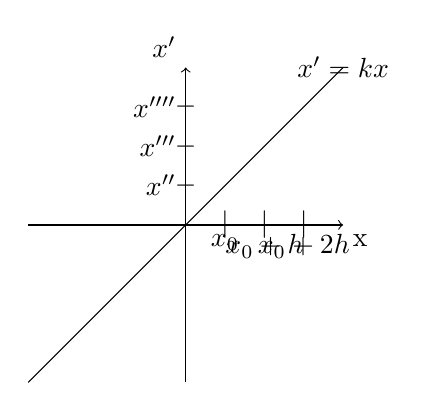
\begin{tikzpicture}[scale=1] %[x={10.0pt},y={10.0pt}]
	\pgfmathsetmacro\MAX{2}
	\draw[->] (-\MAX,0) -- (\MAX,0) node[anchor=north west] {x};
	\draw[->] (0,-\MAX) -- (0,\MAX) node[anchor=south east] {$ x'$};
	\draw[domain=-2:2,smooth,variable=\x] plot ({\x},{\x}) node {$ x'=kx$};
	\draw node at (0.5,0) {$|$};
	\draw node at (1,0) {$|$};
	\draw node at (1.5,0) {$|$};
	\draw node at (0,0.5) {$-$};
	\draw node at (0,1) {$-$};
	\draw node at (0,1.5) {$-$};
	\draw node[anchor=north] at (0.5,0) {$x_0$};
	\draw node[anchor=north] at (1,0) {$x_0+h$};
	\draw node[anchor=north] at (1.5,0) {$x_0+2h$};
	\draw node[anchor=east] at (0,0.5) {$ x'' $};
	\draw node[anchor=east] at (0,1) {$ x''' $};
	\draw node[anchor=east] at (0,1.5) {$ x''''$};
	
	\end{tikzpicture}% pic 1
	\qquad % <----------------- SPACE BETWEEN PICTURES
	\begin{tikzpicture}[scale=1] %[x={10.0pt},y={10.0pt}]
	\pgfmathsetmacro\MAX{2}
	\draw[->] (-\MAX,0) -- (\MAX,0) node[anchor=north west] {t};
	\draw[->] (0,-\MAX) -- (0,\MAX) node[anchor=south east] {x};
	\end{tikzpicture}% pic 2
\end{center}

blablabla ....\\
.......\\
Limiti di questo modello:
\begin{itemize}
	\item la variabile $x$ dovrebbe variare in $\N$, poiché una popolazione ha un numero intero di elementi.
	\item In molte specie è verosimile che il numero di nati al tempo $t$ dipenda dalla popolazione presente ad un tempo precedente $x(t-T), T>0$
	\item Supporre che una popolazione abbia per sempre a disposizione risorse sufficienti può non essere realistico
	\item Questo modello va bene quando si considerano intervalli di tempo molto lunghi.
\end{itemize}